%%%%%%%%%%%%%%%%%%%%%%%%%%%%%%%%%%%%%
% Inlucudings:                      %
%%%%%%%%%%%%%%%%%%%%%%%%%%%%%%%%%{{{%
\documentclass[11pt,english,a4paper,chapterprefix]{scrartcl}
%\usepackage[T1]{fontenc}
\usepackage[bigcaptions]{listing}
%\usepackage[latin1]{inputenc}
\usepackage[small,bf,hang]{caption}
\usepackage[english]{babel}
%\usepackage{epsfig}
\usepackage{wrapfig}
%\usepackage{caption}
\usepackage{psfrag}
\usepackage[rflt]{floatflt}
\usepackage[usenames]{color}
\usepackage{graphicx}
\emergencystretch = 10pt
\usepackage{amsmath}
\usepackage{amssymb}
\usepackage{setspace}
%\usepackage{calc}
\usepackage{tocloft}
\usepackage{listing}
\usepackage{listings}
\usepackage{trsym}
\usepackage{trfsigns}
\usepackage{minted}
\usepackage{multirow}
\usepackage{fancyhdr}
\usepackage{nomencl}
\usepackage{todonotes}
%\usepackage{float}
\usepackage{subfig}
\usepackage[hyphens]{url}
\usepackage{hyperref}
\usepackage{eurosym}
\usepackage{enumitem}
% for solidity-highlighting.tex
\usepackage{listings, xcolor}
% Copyright 2017 Sergei Tikhomirov, MIT License
% https://github.com/s-tikhomirov/solidity-latex-highlighting/

\definecolor{verylightgray}{rgb}{.90,.90,.90}
\definecolor{commentgreen}{rgb}{0.25,0.5,0.35}
\definecolor{stringred}{rgb}{0.6,0,0}

\lstdefinelanguage{Solidity}{
	keywords=[1]{anonymous, assembly, assert, balance, break, call, callcode, case, catch, class, constant, continue, constructor, contract, debugger, default, delegatecall, delete, do, else, emit, event, experimental, export, external, false, finally, for, function, gas, if, implements, import, in, indexed, instanceof, interface, internal, is, length, library, log0, log1, log2, log3, log4, memory, modifier, new, payable, pragma, private, protected, public, pure, push, require, return, returns, revert, selfdestruct, send, solidity, storage, struct, suicide, super, switch, then, this, throw, transfer, true, try, typeof, using, value, view, while, with, addmod, ecrecover, keccak256, mulmod, ripemd160, sha256, sha3, abi}, % generic keywords including crypto operations
	keywordstyle=[1]\color{blue}\bfseries,
	keywords=[2]{address, bool, byte, bytes, bytes1, bytes2, bytes3, bytes4, bytes5, bytes6, bytes7, bytes8, bytes9, bytes10, bytes11, bytes12, bytes13, bytes14, bytes15, bytes16, bytes17, bytes18, bytes19, bytes20, bytes21, bytes22, bytes23, bytes24, bytes25, bytes26, bytes27, bytes28, bytes29, bytes30, bytes31, bytes32, enum, int, int8, int16, int24, int32, int40, int48, int56, int64, int72, int80, int88, int96, int104, int112, int120, int128, int136, int144, int152, int160, int168, int176, int184, int192, int200, int208, int216, int224, int232, int240, int248, int256, mapping, string, uint, uint8, uint16, uint24, uint32, uint40, uint48, uint56, uint64, uint72, uint80, uint88, uint96, uint104, uint112, uint120, uint128, uint136, uint144, uint152, uint160, uint168, uint176, uint184, uint192, uint200, uint208, uint216, uint224, uint232, uint240, uint248, uint256, var, void, ether, finney, szabo, wei, days, hours, minutes, seconds, weeks, years},	% types; money and time units
	keywordstyle=[2]\color{teal}\bfseries,
	keywords=[3]{block, blockhash, coinbase, difficulty, gaslimit, number, timestamp, msg, data, gas, sender, sig, value, now, tx, gasprice, origin},	% environment variables
	keywordstyle=[3]\color{violet}\bfseries,
	identifierstyle=\color{black},
	sensitive=false,
	comment=[l]{//},
	morecomment=[s]{/*}{*/},
	commentstyle=\color{commentgreen}\ttfamily,
	stringstyle=\color{stringred}\ttfamily,
	morestring=[b]',
	morestring=[b]"
}

\lstset{
	language=Solidity,
	backgroundcolor=\color{verylightgray},
	extendedchars=true,
	basicstyle=\footnotesize\sffamily,
	showstringspaces=false,
	showspaces=false,
	numbers=left,
	numberstyle=\footnotesize,
	numbersep=9pt,
	tabsize=2,
	breaklines=true,
	showtabs=false,
	captionpos=b,
	framexleftmargin=5pt
}
\lstset{columns=fullflexible}

%\input{subsections.sty}
\setcounter{secnumdepth}{5}
\setcounter{tocdepth}{5} 
\numberwithin{equation}{section}
\numberwithin{figure}{section}

%%%%%%%%%%%%%%%%%%%%%%%%%%%%%%%%%}}}%
% New Commands and Configurations:  %
%%%%%%%%%%%%%%%%%%%%%%%%%%%%%%%%%{{{%
%\setkomafont{section}{\Large\rmfamily}
%\setkomafont{subsection}{\large\rmfamily}
%\setkomafont{subsubsection}{\normalsize\rmfamily}
\setkomafont{paragraph}{\footnotesize}
\numberwithin{table}{section}
\numberwithin{listing}{section}
\setlength\textheight{24cm}
\definecolor{orange}{rgb}{1 , 0.5 , 0}
\definecolor{blue}{rgb}{0, 0 , 1}
\definecolor{green}{rgb}{0, 1 ,0}
\newcommand{\cb}{\textcolor{blue}}
\newcommand{\subsubsubsection}{\paragraph}
\newcommand{\subsubsubsubsection}{\subparagraph}
\clubpenalty = 10000
\widowpenalty = 10000
\displaywidowpenalty = 10000
\parindent0pt % No Indent
\makenomenclature
% Document Head
\begin{document}
%\restylefloat{figure}
\pagestyle{fancy}
\rhead{} 

\definecolor{light-gray}{gray}{0.90}

%\lstset{ %
%language=C,                % choose the language of the code
%basicstyle=\small\ttfamily
%,       % the size of the fonts that are used for the code
%%numbers=left,                   % where to put the line-numbers
%numberstyle=\footnotesize,      % the size of the fonts that are used for the line-numbers
%stepnumber=2,                   % the step between two line-numbers. If it's 1 each line 
%                                % will be numbered
%numbersep=5pt,                  % how far the line-numbers are from the code
%backgroundcolor=\color{light-gray},  % choose the background color. You must add \usepackage{color}
%showspaces=false,               % show spaces adding particular underscores
%showstringspaces=false,         % underline spaces within strings
%showtabs=false,                 % show tabs within strings adding particular underscores
%frame=single,                   % adds a frame around the code
%rulecolor= \color{light-gray},
%tabsize=2,                      % sets default tabsize to 2 spaces
%captionpos=b,                   % sets the caption-position to bottom
%breaklines=true,                % sets automatic line breaking
%breakatwhitespace=false,        % sets if automatic breaks should only happen at whitespace
%title=\lstname,                 % show the filename of files included with \lstinputlisting;
%                                % also try caption instead of title
%escapeinside={\%*}{*)},         % if you want to add a comment within your code
%xleftmargin=1cm,
%xrightmargin=1cm,
%morekeywords={*,...}            % if you want to add more keywords to the set
%}
%
\newminted{perl}{linenos, bgcolor=light-gray, fontsize=\scriptsize}
\newminted{cpp}{bgcolor=light-gray, fontsize=\scriptsize}
\newminted{tcl}{bgcolor=light-gray, fontsize=\scriptsize}
\newminted{sh}{bgcolor=light-gray, fontsize=\scriptsize}
\newminted{basemake}{bgcolor=light-gray, fontsize=\scriptsize}

%%%%%%%%%%%%%%%%%%%%%%%%%%%%%%%%%}}}%
% fancy nomenclautur:
%%%%%%%%%%%%%%%%%%%%%%%%%%%%%%%%%{{{%
%\setlength{\nomlabelwidth}{.20\hsize}
%\renewcommand{\nomlabel}[1]{#1 \dotfill}

%<*sample05>
\def\@@@nomenclature[#1]#2#3{%
 \def\@tempa{#2}\def\@tempb{#3}%
 \protected@write\@nomenclaturefile{}%
  {\string\nomenclatureentry{#1\nom@verb\@tempa @[{\nom@verb\@tempa}]%
    |nompageref{\begingroup\nom@verb\@tempb\protect\nomeqref{\theequation}}}%
    {\thepage}}%
 \endgroup
 \@esphack}
%\def\nompageref#1#2{%
%  \if@printpageref\pagedeclaration{#2}\else\null\fi
%  \linebreak#1\nomentryend\endgroup}
\def\pagedeclaration#1{\dotfill\nobreakspace ~#1}
%\def\nomentryend{.}
\def\nomlabel#1{\textbf{#1}\hfil}
\makeatletter 
\renewcommand*\dotfill{\leavevmode% 
  \leaders\hbox{$\m@th 
  \mkern \@dotsep mu\hbox{.}\mkern \@dotsep 
  mu$}\hfill\kern\z@} 
\makeatother
%%%%%%%%%%%%%%%%%%%%%%%%%%%%%%%%%}}}%
% Abbr Commands!
%%%%%%%%%%%%%%%%%%%%%%%%%%%%%%%%%{{{%
\newcommand{\abbr}[2]{\textit{#2} (#1)\nomenclature{#1}{#2 \nomrefpage}}
\newcommand{\shortabbr}[2]{\nomenclature{#1}{#2 \nomrefpage}}
\newcommand{\revabbr}[2]{#1 (\textit{#2})\nomenclature{#1}{#2 \nomrefpage}}

%%%%%%%%%%%%%%%%%%%%%%%%%%%%%%%%%}}}%
% Titlepage                         %
%%%%%%%%%%%%%%%%%%%%%%%%%%%%%%%%%{{{%
%%%%%%%%%%%%%%%%%%%%%%%%%%%%%%%%%%%%%%%%%%%%%%%%%%%%%%%%%%%%%%%%%%%%%%%%%%%%%%%%%%%%%%%%%%%%%%%%%%%
\begin{titlepage}
\setcounter{page}{-3}
\begin{center}
\includegraphics*[scale=2.5]{img/TUKL_LOGO.pdf}\\[3ex]

\textsc{\Large University of Kaiserslautern}\\[1.5ex]
Department of Electrical Engineering and Information Technology\\[1.5ex]
Microelectronic Systems Design Research Group \\[3ex]

\vfill
\vfill

\textsc{\Huge Bachelor Thesis}\\[6ex]
\centerline{\Large Design and Implementation of a Blockchain-Based Smart Outlet Concept}
\vspace{20pt}
\centerline{\Large Entwurf und Implementierung eines Blockchain-basierten Smart Outlet Konzepts}

\vfill
\vfill

 \begin{tabular}{rl}\hline\\
 Presented:                & \quad \today \\[1.5ex]
 Author:                   & \quad Daniel Gretzke (392488) \\[1.5ex]
 Research Group Chief:     & \quad Prof.\,Dr.-Ing.\,~N.~Wehn\\[1.5ex]
 Tutor:                    & \quad M.Sc. Frederik Lauer\\[1.5ex]\\\hline
 \end{tabular}
\end{center}

    \clearpage
    \pagestyle{empty}
    \begin{flushleft}
    \section*{Statement}
    \vspace{10mm}
    I declare that this thesis was written solely by myself and exclusively with
    help of the cited resources.

    \vspace{12pt}
    Kaiserslautern, \today \\
%    Kaiserslautern, XXst XXXXXX 2010 \\
    \vspace{20mm}
    Daniel Gretzke
    \end{flushleft}

\end{titlepage}


\newpage
%%%%%%%%%%%%%%%%%%%%%%%%%%%%%%%%%}}}%
% Abstract                          %
%%%%%%%%%%%%%%%%%%%%%%%%%%%%%%%%%{{{%
\onehalfspacing % Stelle 1.5er Abstand ein
\newpage
\thispagestyle{empty}

\section*{Abstract}

\textcolor{red}{Abstract English here.}
\newpage
\thispagestyle{empty}

\section*{Zusammenfassung}

\textcolor{red}{Zusammenfassung Deutsch hier.}
\newpage
%%%%%%%%%%%%%%%%%%%%%%%%%%%%%%%%%}}}%
% Table of Contents                 %
%%%%%%%%%%%%%%%%%%%%%%%%%%%%%%%%%{{{%
\tableofcontents
\newpage
%\setcounter{page}{1}
\newpage
%%%%%%%%%%%%%%%%%%%%%%%%%%%%%%%%%}}}%
% Chapters                          %
%%%%%%%%%%%%%%%%%%%%%%%%%%%%%%%%%{{{%
\onehalfspacing % Stelle 1.5er Abstand ein
%\setstretch{1.1} 
\section{Introduction}
\begin{quote}
  Whereas most technologies tend to automate workers on the periphery doing menial tasks, blockchains automate away the center. Instead of putting the taxi driver out of a job, blockchain puts Uber out of a job and lets the taxi drivers work with the customer directly.
  \\
  {\textit{— Vitalik Buterin, co-founder of Ethereum}}
\end{quote}

A cryptocurrency based on a blockchain was first implemented in 2009 by Satoshi Nakamoto (pseudonym) and was called Bitcoin.
Since then, it has steadily gained importance every year.
Meanwhile, thousands of cryptocurrencies and tokens were built on this technology.
The hype in the year 2017 called the attention of many companies to blockchain and even last year, when the value of cryptocurrencies fell as far as 95\%, the interest in this field did not drop.
\\\\
Compared to traditional payment methods like Visa, Banks and PayPal, cryptocurrencies are built decentralized, meaning that there is no central organization that controls transactions, the issuance of new money, et cetera.
The validity of the blockchain \abbr{peer to peer}{P2P} network is secured through cryptographic protocols.
This brings several benefits.
Traditional payment methods usually go with high transactions costs, most commonly in the amount of a few percent.
On the contrary, the cost of a single transaction on a blockchain averages out at just a few cents\cite{ethereum-fee}.
Some cryptocurrencies even work without any fees.
\\\\
Because of this, they are suited for micro transactions really well.
There are some disadvantages, though.
The blockchain technology is still at an early stage and really immature.
Compared to traditional electronic payments, it only manages to achieve very few \abbr{transactions per second}{TPS} and has long transaction times.
E.g., Bitcoin manages 4-5 TPS\cite{bitcoinTPS} as opposed to Visa, which manages to process almost 4,000 TPS on average\cite{visa}.
\\\\
As stated in the quote above, the key strength of blockchain and cryptocurrencies is the decentralization aspect.
For many, it will reshape various markets we know today, potentially revolutionize the financial industry and even disrupt monopolies in the future.
\\\\
Another trend regarding the future are electric cars.
It's expected that in a few years most cars on the road and almost all cars sold will be electric.
Often these need to be charged overnight.
Unfortunately, most city residents are familiar with the problem that they rarely park in front of their own house, let alone own a garage.
It's foreseeable that recharging your car might bring difficulties.
\\\\ 
This bachelor thesis is devoted to this problem.
It examines whether a smart electrical socket, which is placed outside the house by a homeowner, can be used to efficiently sell electricity and which payment method is suited best for this task.
Based on an initial concept, a prototype is to be developed that implements the previously worked out features.
It will serve as an example on how to implement \abbr{machine to machine}{M2M} payments on a microcontroller level.
\newpage
\clearpage
\section{Theory}
The purpose of this chapter is to explain the most important terms about blockchain and the key underlying components of the technology. Most explanations will be kept superficial, as the technological implementation is too complex to deal with it in a few sentences.
\\\\

\textbf{Hash}\\
The cryptographic hash function is a mathematical function that usually fulfills the following requirements\cite{hash}:
\begin{enumerate}
    \item determinism: the same input always produces the same output
    \item preimage resistance: it’s nearly impossible to get the input from the output
    \item second-preimage resistance: it’s nearly impossible to find a second input that produces the same output as the first input
\end{enumerate}
The output of this function is called hash. Bitcoin uses the SHA-256\cite{bitcoin-whitepaper}, Ethereum uses the Keccak-256\cite{ethereum-yellow-paper} hashing algorithm which produces an output hash with a length of 32 bytes.
\\\\

\textbf{Public Key Cryptography}\\
Public key cryptography\cite{public-key-cryptography} is the backbone of the blockchain technology and consists of a key pair – a private and a public key. As the name suggests the private key needs to be secret and the public key can be shared with anyone. A message can be signed using the private key resulting in a signature. This signature can then be verified using the public key to prove that the message was, in fact, signed by the corresponding private key. Bitcoin and Ethereum use the \abbr{Elliptic Curve Digital Signature Algorithm}{ECDSA} for signatures. They are used to prove that transactions were really sent by a specific account and not manipulated.
\\\\

\textbf{Wallet}\\
Everything that’s needed to send and/or receive cryptocurrencies is a private key\cite{bitcoin-whitepaper}, meaning a private key is a wallet in it’s simplest form. More complex forms of a wallet encrypt a private private key with a password or store it on a dedicated hardware device.
\\\\

\textbf{Address}\\
An address is used to identify participants on the blockchain and usually is the public key belonging to the private key of the account or is generated fromm the public key, e.g. Ethereum  uses the right most 20 bytes of the hash of the public key as the address\cite{ethereum-yellow-paper}.
\\\\

\textbf{Ledger}\\
The equivalent of a traditional Record of all addresses and their balances. Every participant of the network has a copy of this Ledger.
\\\\

\textbf{Node}\\
A node is a participant on the blockchain. When a new node joins the network, it downloads the ledger, currently accepted by the majority. A so-colled full node has the entire history of the ledger – from the first block, to the latest.
\\\\

\textbf{Transaction}\\
A transaction updates the Ledger, e.g. reducing the balance of an address by a specific amount and adding it to the balance of another account.
\\\\

\textbf{Blockchain}\\
A list of transactions is bundled together into a block. Also included in this block is the hash of the previous block, which contains the hash of the previous block, and so on and creates a chain of blocks\cite{bitcoin-whitepaper} which always point to their predecessor, thus the name blockchain. This is also the reason why a blockchain is considered immutable: modifying any information in a block would automatically change the hashes of every block after it and would be rejected by the network.
\\\\

\textbf{Miner / Validator}\\
A participant of the network whose task it is to secure the network and validate / mine new transactions and blocks.
\\\\

\textbf{Proof of Work}\\
There are different approaches to reach consensus over which block should be added next to the network, \abbr{Proof of Work}{PoW} is one of them and is used by most cryptocurrencies. A \abbr{number used once}{nonce} is included in the block which is adjusted by a validator. Every different nonce produces a different block hash. The goal is to find a nonce that is numerically lower than a certain threshold value (also called difficulty). A validator who finds this number can submit their block to the network. All miners race to find the nonce as fast as possible, so their block will be accepted by all other participants in the network and considered valid. The fastest submission gets a so-colled block reward, a reward minted by the protocol to the fastest miner and all transaction fees from that block.
\\\\

\textbf{Block Time}\\
The time it takes to add a new block to the network is called block time. On the Bitcoin network the block time is 10 minutes\cite{bitcoin-whitepaper}, Ethereum wants to archive a block time of 12 seconds\cite{ethereum-blocktime}, realistically its averaging at about 15 seconds\cite{ethereum-blocktime-chart}. The difficulty is adjusted automatically to keep the block time roughly the same, no matter how much computing power is currently mining.
\\\\

\textbf{Confirmation Time}\\
The time it takes until a transaction is mined. The higher the transaction fee the faster transaction is confirmed.
\\\\

\textbf{Ethereum Virtual Machine}\\
The \abbr{Ethereum Virtual Machine}{EVM} is a turing complete virtual machine that can execute computer code on the Ethereum Blockchain. As a result the Ethereum network acts like a decentralized computer with all the features of a blockchain: the storage is entirely public and every computation or code execution is recorded on the blockchain.
\\\\

\textbf{Smart Contract}\\
Smart contracts are written in special programming languages, the most popular being called "Solidity", and are compiled into bytecode afterwards. This bytecode is then publicly stored on the blockchain and can be executed by everyone. The advantage of smart contracts is, that the code is public to everyone and immutable, thus can theoretically be used as a binding, programmable contract that can control monetary value on its own. As a drawback every computational step and byte stored on the blockchain costs money in form of transaction cost.
\\\\

\textbf{DApp / Web3}\\
DApp stands for decentralized application. Web3 is also called the decentralized web, where websites are powered by smart contracts and DApps. 
\\\\

\textbf{Account}\\
There are two types of accounts on the Ethereum Blockchain: An \abbr{externally owned account}{EOA} and a contract account. Each of those accounts has a transaction count and a balance\cite{ethereum-yellow-paper} associated with them. An EOA is controlled by a private key, whereas a contract account has code and storage associated with it.
\\\\

\textbf{Off-chain Transactions / Payment Channels}\\
For every transaction on the blockchain fees have to be paid. One way to save transaction costs is to have multiple transactions that are not recorded on the blockchain, so-colled off-chain transactions, and settle them on the blockchain, once the payment process is finished.
\\\\

\textbf{Ether - Gwei - Wei}\\
Ether is the currency used on the Ethereum network. It can be divided into smaller fractions. The most important are Wei and GWei. Wei is the smallest unit: 1 Ether equals \(10^{18}\) Wei\cite{ethereum-yellow-paper}. Gwei is primarily used for calculations of transaction costs: 1 Ether equals \(10^{9}\) Gwei, 1 Gwei equals \(10^{9}\) Wei. Ether is always used in Wei format in Smart Contracts.
\\\\

\textbf{Mainnet / Testnet}\\
The main network of a blockchain is called the Mainnet. Testnets are blockchain networks that behave the same way as the Mainnet. This allows developers to develop smart contracts without the risk of losing any monetary value. Additionaly, improvements to the Mainnet are often tested on a Testnet prior to their official implementation.
\newpage
\clearpage
\section{Concept}
This section describes the requirements for the overall concept and goals of this bachelor thesis, analyzes different payment methods to evaluate which meet said requirements and defines a concept and its hardware requirements for a possible implementation.
\\
\subsection{Definition of Prerequisites}

The following prerequisites are required to develop a concept for the sale of electricity between two parties who do not know each other:
\begin{enumerate}
    \item A potential customer Alice owns an electric car and wants to purchase electricity to charge it overnight.
    \item A supplier Bob who owns a smart electrical socket wants to sell electricity.
    \item Alice and Bob do not meet, Alice does not trust Bob to supply the electricity she paid for, Bob does not trust Alice to not wrongfully revert the payment after the electricity has been supplied.
    It has to be assumed that there are bad actors, who want to steal from the other party (in the form of monetary value or electricity).
    \item For all calculations throughout this thesis the following values are assumed:
    \begin{enumerate}
        \item Charging power: 3.7 kW
        \item Electricity price: 0.3 \euro/kWh
        \item Total transferred energy: 40 kWh
        \item Charging duration: 11 hours
        \item Electricity cost: 12 \euro
        \item Price for the customer: 18 \euro{} (profit margin of 50\%)
    \end{enumerate}
\end{enumerate}
\leavevmode
\\
The objective of this chapter is to evaluate which payment method is suited best for the described use case.
Next, the goals of the M2M payment system have to be defined:

\begin{enumerate}
    \item Value has to be transferred from Alice to Bob.
    \item Electricity has to be supplied in return for a payment, whereby the risk or impact of not getting electricity in return has to be minimal.
    \item Alice needs to be able to stop paying for electricity when it is not longer needed, e.g., when the battery is fully charged, without overpaying.
    \item Bob should only start supplying electricity after a valid payment was received and thus the risk of losing electricity is minimized.
    \item Value should be transferred from Alice to Bob at least once per minute to continuously pay for electricity to reduce risk, but transaction fees should stay at a minimum at the same time.
    For this thesis a payment interval of 15 seconds is assumed resulting in 0.007 \euro{} per payment.
    \item All calculations relevant for the payment system should be able to be processed on an embedded platform with low computational power and memory.
\end{enumerate}
\leavevmode
\\
\subsection{Analysis of Different Payment Methods}
In this subsection, the advantages and disadvantages of traditional payment methods, established electronic and online payments and cryptocurrencies are compared and a payment method for the implementation is chosen.
\\
\subsubsection{Traditional Currency}
The simplest form of monetary value is cash, it could be imagined that money could be paid through a coin slot and electricity would be returned as a result.
It's not suitable for this use case, as the risk of not receiving any electricity in return for the customer and the risk of theft for the supplier, e.g., someone violently stealing the cash, is too high.
\\\\
Traditional electronic or online payments like VISA or PayPal pose a low risk of theft for the buyer because of customer protection methods, unfortunately, the risk for the seller is non-negligible, e.g., in the form of credit card fraud or customer protection exploitation.
Another disadvantage can be seen in the high fees, PayPal, for example, has a pricing of 0.10 \euro{} + 10\% for micro-transactions\cite{paypal-fees} and wouldn't be economically feasible for the predefined goals.
The key strength is a fast, near-instant transaction time.
\\
\subsubsection{Cryptocurrency}
Cryptocurrency payments have some major advantages over the previously analyzed payment methods.
Compared to electronic and online payments, many cryptocurrencies have lower fees and some even work without any fees at all.
Payments can be broken down into fractions, as mentioned above, with payment intervals of a minute or less.
Because all payments are immutable, the supplier has no risk and the customer risks just losing less than one cent for a first payment.
Additionally the currency can be stored right on an embedded device and the machine is in charge of sending transactions.
One of the biggest disadvantages of cryptocurrencies for M2M payments are long transaction times, but as the technology is still in its infancy, this might change in the future.
\\\\
Over a thousand different cryptocurrencies exist\cite{coincap} and every one of them has their own rules that can drastically differ from the next one.
Each underlying blockchain technology has their benefits and drawbacks.
In the next paragraphs, some of these digital currencies will be evaluated whether or not they are suitable to reach the set goals.
\\\\\\
\textbf{Bitcoin}\\
Because Bitcoin is the earliest cryptocurrency, it suffers from problems other cryptocurrencies could improve upon.
As demonstrated in Figure \ref{fig:BitcoinConfirmationTime}, scalability is one of these issues.
The block time is 10 minutes\cite{bitcoin-whitepaper} and during peak times the average confirmation time can take more than two hours.
Thus bitcoin should not be considered for this use case.
\\
\begin{figure}[H]
    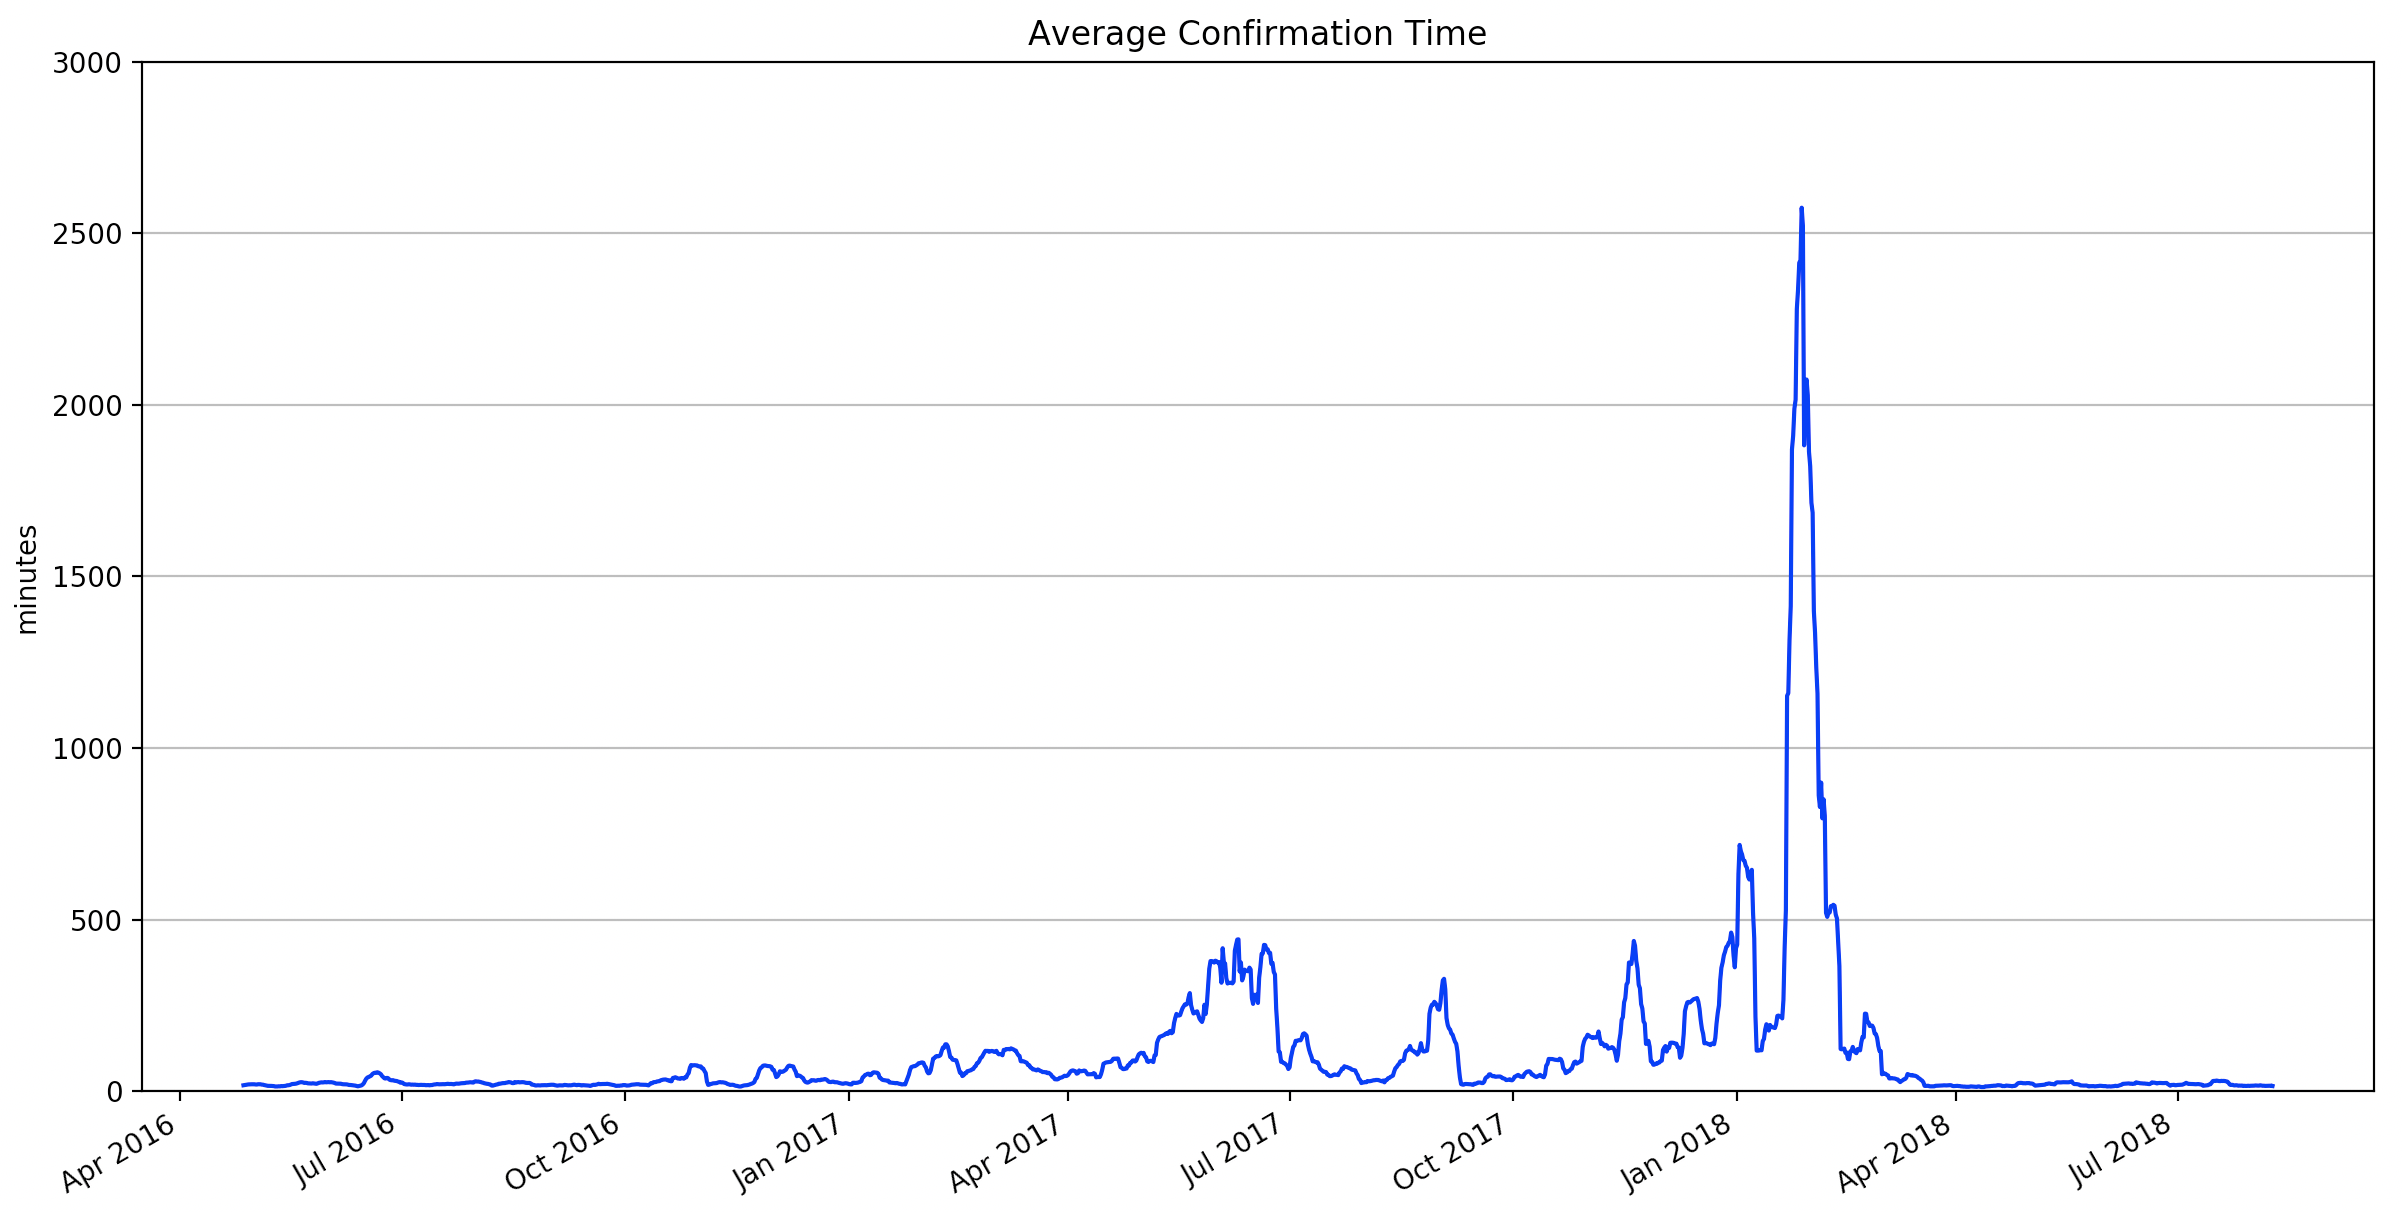
\includegraphics[width=\textwidth]{img/average-confirmation-time.png}
    \caption{Average confirmation time of a transaction on the Bitcoin blockchain\cite{btc-conf-time}}
    \label{fig:BitcoinConfirmationTime}
\end{figure}
\leavevmode
\\
\textbf{IOTA}\\
As previously mentioned, there are some cryptocurrencies that work without any fees that are worth to be considered.
One of these currencies is IOTA.
It was designed especially with M2M payments in mind and the underlying technology, called Tangle, differs from traditional blockchains.
The way it works is that before someone's transaction can be validated, they need to validate other transactions first\cite{tangle}.
In theory, this makes the network scale especially well — the more transactions are broadcasted, the shorter the transaction times get.
In practice, transaction times are at 2.6 minutes at the time of writing\cite{iota-time} and therefore not fast enough for this use case.
\newpage
\textbf{Nano}\\
Another feeless cryptocurrency is called Nano, formerly known as RaiBlocks.
It is built upon a technology called block-lettuce.
Each account on the network is an independent blockchain which can update itself asynchronously from the rest of the accounts.
This makes Nano not only have zero transaction fees but also allows it to have transaction times of less than a second.
It can also handle way more TPS than Bitcoin and Ethereum, namely around 100 TPS over a longer period of time with peaks up to 300 TPS\cite{nano-stress-test}.
\\\\
Unfortunately, at the time of development of the prototype, the Nano network faced some issues which resulted in transaction times in up to 20 seconds, as seen in Figure \ref{fig:NanoConfirmationTime}.
After the V18 update these problems were solved and the transaction times returned back to less than a second\cite{nano-confirmation-time}.
\begin{figure}[H]
    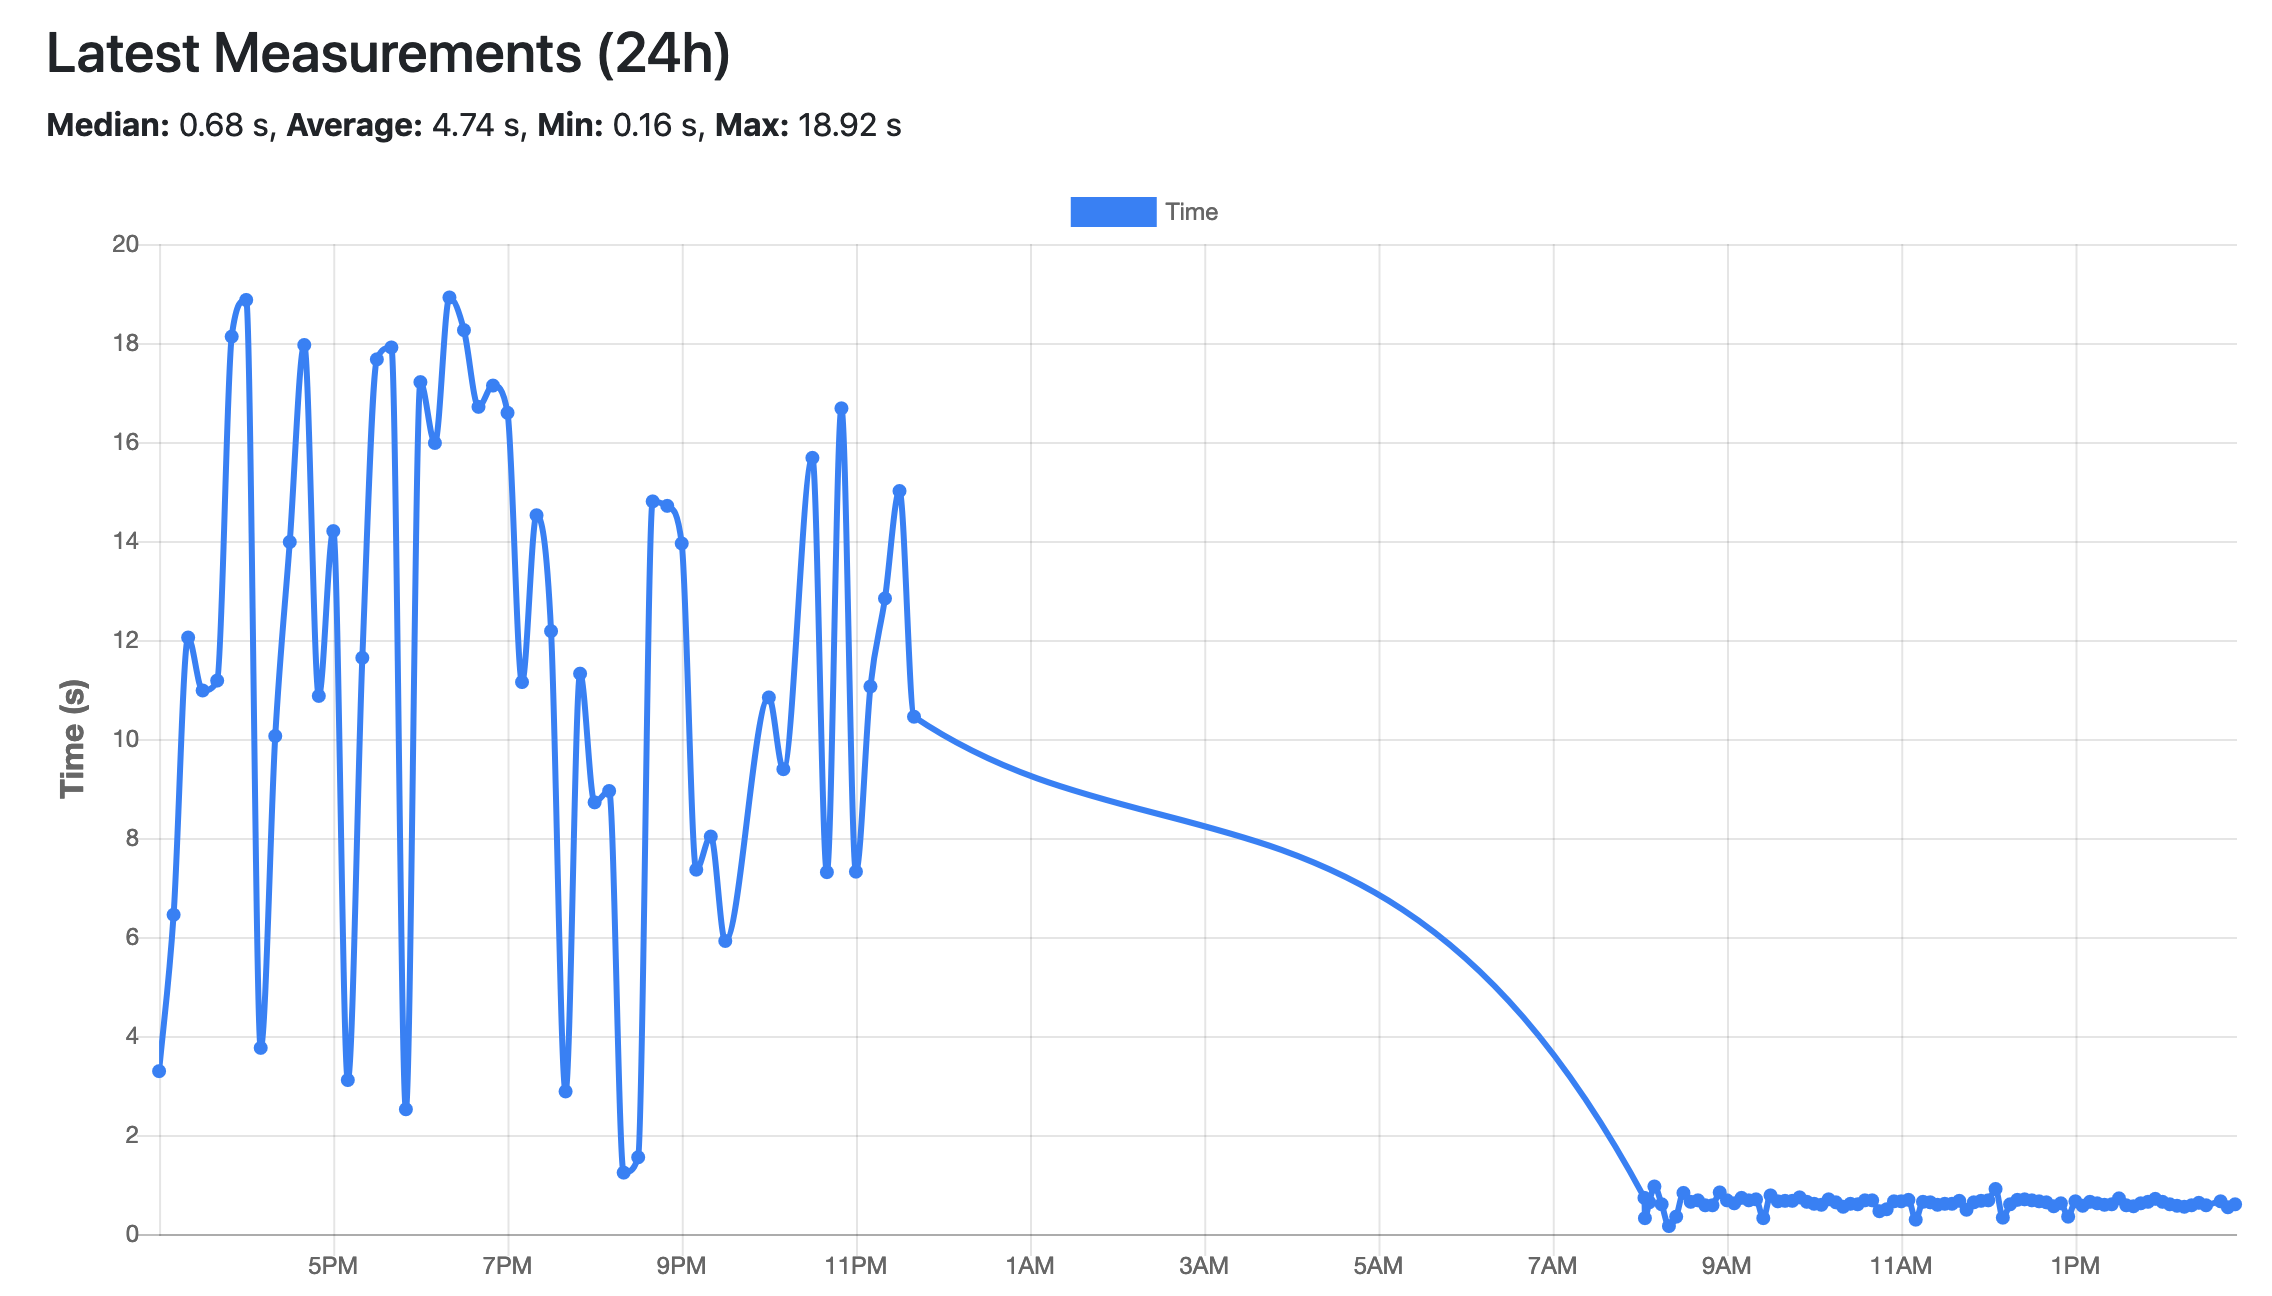
\includegraphics[width=\textwidth]{img/nano-confirmation-time.png}
    \caption{Improvements of transaction times after the update to V18 on Feb. 22nd, 2019\cite{nano-confirmation-time}}
    \label{fig:NanoConfirmationTime}
\end{figure}
Although the currency was considered at first, the main reason Nano was not chosen for the implementation is that it was not built with M2M transactions in mind.
To prevent spamming, i.e., attacking the network through congesting it with transactions, PoW needs to be generated in order to send or receive transactions.
According to the Nano white paper\cite{nano-white-paper} an Intel Core i7-4790K processor with 4.00 GHz can handle up to 0.33 TPS.
A microcontroller would not be able to generate the PoW required for the transactions in a reasonable amount of time.
Instead, a dedicated server would be required for each supplier and customer, which would store the private keys and handle the transmission and reception of transactions.
The micro controllers would merely communicate with said servers and therefore the currency did not meet the defined requirements.
\newpage
\textbf{Ethereum}\\
Ethereum has a block time of 15 seconds.
At the time of writing the fee to be included in the next block is 0.01 \euro\cite{ethereum-fee}.
In this case, the transaction would be fast enough to meet the goal of 4 transactions per minute, but the transaction fees would exceed the payment, raising the total price as much as 143\%.
\\\\
One way to cut transaction fees is the use of off-chain transactions.
As previously mentioned, these work very similarly to on-chain transactions: information like a beneficiary and value can be signed by a sender, so it can be proven where the transaction originates from.
They differ from each other, as off-chain transactions are not recorded on the blockchain.
They can be sent from one participant to another directly, therefore there is no transaction fee or transaction time involved.
A number of these off-chain transactions can be bundled in a payment channel.
In the end, these transactions have to be settled on the blockchain, actually modifying the ledger and updating the balances of all participants.
Thus the 2,460 transactions required during a charging period of 11 hours can be bundled into a few transactions on the blockchain.
Sending on- and off-chain transaction requires computations like encoding, hashing or signing of data which can be achieved on an embedded platform.
Therefore this payment method meets all the requirements listed above.
\\\\
Ethereum was chosen for the implementation of this prototype, as it implements a virtual machine with the ability to execute code, therefore a payment channel can be built using smart contracts.
The following steps briefly explain how the payment concept works:
\\
\begin{enumerate}
    \item The customer places a deposit (max. purchase value) into the smart contract and initializes the payment channel.
    \item The customer signs an off-chain transaction and sends it to the supplier.
    \item Once the supplier receives the transaction, the delivery of electricity begins.
    Steps 2 \& 3 are repeated until the customer or the supplier want to discontinue the exchange.
    \item As soon as any party wants to close the payment channel, the supplier submits the offline transactions to the smart contract.
    Each party is now able to withdraw their share from the smart contract.
\end{enumerate}
\begin{figure}[H]
  \begin{center}
    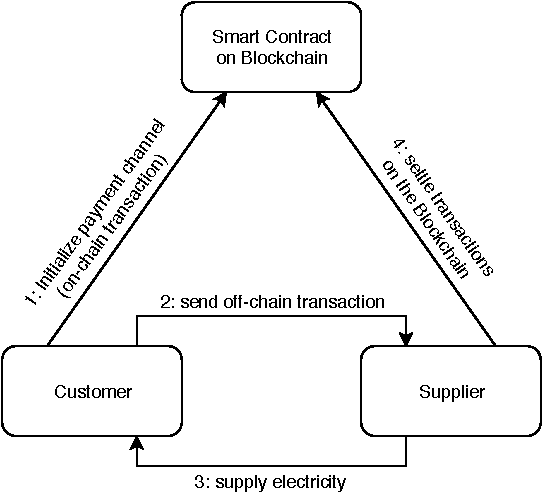
\includegraphics[height=8cm]{img/payment_channel.pdf}
    \caption{Sketch of a payment channel}
    \label{fig:paymentchannel}
  \end{center}
\end{figure}
With payment channels, the risk of the supplier is minimal, as electricity must only be provided when a valid payment was received and the customer only risks losing one transaction for the initialization of the payment channel and one off-chain transaction if no electricity is provided in return.
\\\\
In total, only 4 transactions have to be made.
One for the payment channel initialization, one for the settlement, and one by each party to withdraw the balances, totaling all transaction fees at a couple cents.
\newpage
\subsection{Component Requirements}
As demonstrated in Figure \ref{fig:concept} the concept is based on four components.
A supplier, a customer, a node in form of a server and a smart contract on the Ethereum blockchain.
\\
\begin{figure}[H]
  \begin{center}
    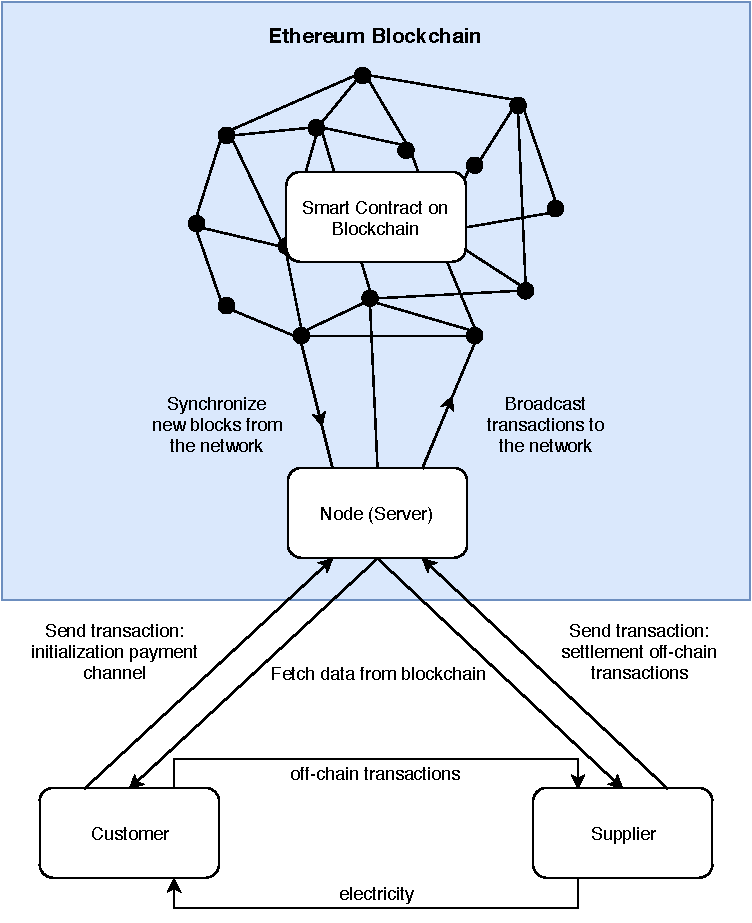
\includegraphics[height=17cm]{img/concept.pdf}
    \caption{Sketch of the concept}
    \label{fig:concept}
  \end{center}
\end{figure}

The supplier should have a microcontroller which is integrated directly into an electrical socket.
This way it can be powered directly by the supplier's circuit and can be protected against external damages, e.g., caused by weather or human influences.
A relay should be placed between the circuit and the socket, which can be switched on and off by the microcontroller to start and stop the supply of electricity to the customer.
For the communication with the Ethereum network an internet connection is required.
It can be either established by connecting to a cellular network using a SIM card or to a WiFi network, preferably of the supplier itself.
\\\\
The customer should have a microcontroller which is integrated into an electrical plug.
If it is integrated into a short extension cord, any electrical device can be connected to it and be charged.
The microcontroller should be able to measure whether electricity is flowing through the cord using a current sensor, e.g., a hall effect-based sensor.
The plug is required to communicate with the Ethereum network as well, therefore a SIM card can be integrated to connect to a cellular network or the plug can use the supplier's WiFi connection for the communication.
The microcontroller can be powered directly by the supplier's socket itself, as the electricity output can be limited to sufficiently power the customer's microcontroller but not enough to charge any device.
\\\\
Both parties are required to communicate with each other, as payment information needs to be exchanged and off-chain transactions need to be sent and received.
The microcontrollers can send information to each other over the circuit itself using \abbr{power-line communication}{PLC} or, if the customer and supplier are using the same WiFi network, it can be used to handle the communication between both parties.
\\\\
The design and functionality of the off-chain transactions is defined by the implementation of the smart contract, which should have the following features.
It should act in the interest of the customer and the supplier, securing both parties from fraud.
A payment channel should be initialized by the customer by depositing an amount of Ether into the smart contract.
The smart contract should act as a trustee, managing the funds until the payment channel is closed again.
The customer can then start signing off-chain transactions with its private key and sending them to the supplier.
When the payment channel is ready to be closed, the supplier should submit the off-chain transactions to the smart contract, as it is in its interest to submit all transactions.
The smart contract is required to verify whether the off-chain transactions were indeed signed by the customer.
If the transactions are valid, the smart contract can then pay out the total transaction volume to the supplier and refund the remainder to the customer.
To ensure that both parties are protected, the payment channel should have an expiration date.
In case the supplier fails to submit a valid signature in a certain amount of time, the customer should be able to withdraw the entire deposit from the smart contract.
\\\\
To initialize and close the payment channel, the customer and the supplier need to be able to communicate with the Ethereum blockchain, which is achieved with a node.
It is the only component required to run on a server, as the entire blockchain history has to be downloaded which takes up several gigabytes of data.
When relevant payment information, e.g., the price per second stored in the smart contract, needs to be fetched from the blockchain, the server sends the information stored in its synchronized local copy.
When data is sent to the blockchain in form of a transaction, the entire process of generating the transaction computes on the microcontroller.
The transaction is then sent to the node which forwards it to the other blockchain participants.
Therefore, the node acts as a gateway between the Ethereum network and the microcontrollers.
\\
\subsection{Risks \& Concerns}
Although choosing payment channels implemented on a blockchain over traditional payment methods brings some advantages in low transaction fees and every party being in charge of their own money, there are some drawbacks that are worth noting:
\\\\
The reason no party has to trust another when using smart contracts is immutability.
Once the code has been deployed to the blockchain, it cannot be changed after the fact.
This poses a risk, as bugs found in the smart contract code cannot be fixed either.
This already resulted in losses of multiple hundreds of millions of dollars on the Ethereum blockchain alone\cite{dao-hack}.
\\
As soon as funds are stored inside a smart contract or on a physical device there is a financial incentive for hackers to try to steal the money.
As the private keys of the customer and supplier are stored on the embedded devices themselves, every part of the microcontroller has to be carefully secured, so under no circumstances the private key can be extracted to steal funds.
Therefore, PLC should be chosen over a WiFi connection for the communication between the customer and the supplier.
\\
Because the concept is designed as a P2P, middleman free system, not only 3rd parties have an incentive to steal funds.
If the customer uses the supplier's WiFi network to communicate with the blockchain, a man in the middle attack should be prevented by using a HTTPS connection secured over TLS.
\\
Transactions are the most secure part of the concept, as they are always digitally signed.
Therefore, even if they are intercepted by a malicious actor, they can only be used for their intended purpose.
\\\\
Another concern is that the concept would not work economically at the time of writing.
Cryptocurrencies and the blockchain technology are still in its infancy and therefore the price is extremely volatile.
A sudden rise or drop of 40\% in price is not rare and would heavily influence the customer experience.
Additionally, only very few people actually own cryptocurrencies and are willing to pay or receive payments using cryptocurrencies.
Because of the low adoption rate, the concept would not be economically feasible as a real product at the time of writing.
\newpage
\subsection{State of the Art}
The exploratory research conducted for this thesis focused on studying concepts and design choices of similar projects completed in the commercial field.
\\\\
A few companies already started researching and experimenting with blockchain technologies and even went as far as combining it with e-mobility.
A company called accessec GmbH built a prototype of a car wallet that works with the IOTA cryptocurrency and integrates a point of sale allowing to conduct transactions with vendors seamlessly\cite{car-wallet}.
Bosch teamed up with the energy supplier EnBW to build a prototype of a blockchain based charging station\cite{bosch-dlt}.
\\\\
The project that came closest to the topic of this bachelor thesis is called Share\&Charge, formerly known as Blockcharge\cite{share-charge}\cite{blockcharge}, which was founded by Innogy, a subsidiary of the energy company RWE\cite{innogy}.
It launched at the end of April 2017 with close to 1,500 charging stations, but the project was closed merely a year later\cite{share-charge-closed}.
It claimed to be a P2P charging network calling itself the "AirBnB of Charging Stations".
It was running on the Ethereum mainnet where anyone could become a charging station owner by purchasing a smart electrical socket to sell electricity.
At first glance it seemed like the solution this bachelor thesis was trying to achieve, but upon further investigation the decentralization aspect had to be questioned.
The electrical socket was communicating with a smartphone app to manage the purchase of electricity.
This app had to be preloaded with fiat currency via PayPal, etc., the transaction was conducted in fiat and a charging station owner could only withdraw fiat currency as well.
There is no evidence that the monetary transaction itself was handled on the blockchain and not just the record aspect of it.
Additionally, it was claimed that the system worked without a middleman but the fee that had to be paid to Share\&Charge with every charging process contradicts that claim.
All this information led to the conclusion that the private keys probably were not handled by the users themselves which is a crucial point in building decentralized applications.
\\\\
To summarize, all projects combining blockchain with e-mobility seem to be bringing existing centralized business models to the blockchain and could work just as well with traditional payment methods.
Furthermore, no technical information, let alone source code, could be found that could be used or improved upon for this bachelor thesis.

\newpage
\clearpage
\section{Implementation}
This chapter will go into the details of the implementation of the previously worked out concept, explain why certain design choices were made as well as all challenges that were faced to successfully implement the payment system on an embedded platform.
\\
\subsection{State Machine}
The concept was implemented on the microcontrollers as finite state machines.
As seen in Figure \ref{fig:state_machine}, the implementation of the payment system is divided into four phases.
Both, the customer and the supplier follow this flowchart for their state machine.
\\
\begin{figure}[H]
  \begin{center}
    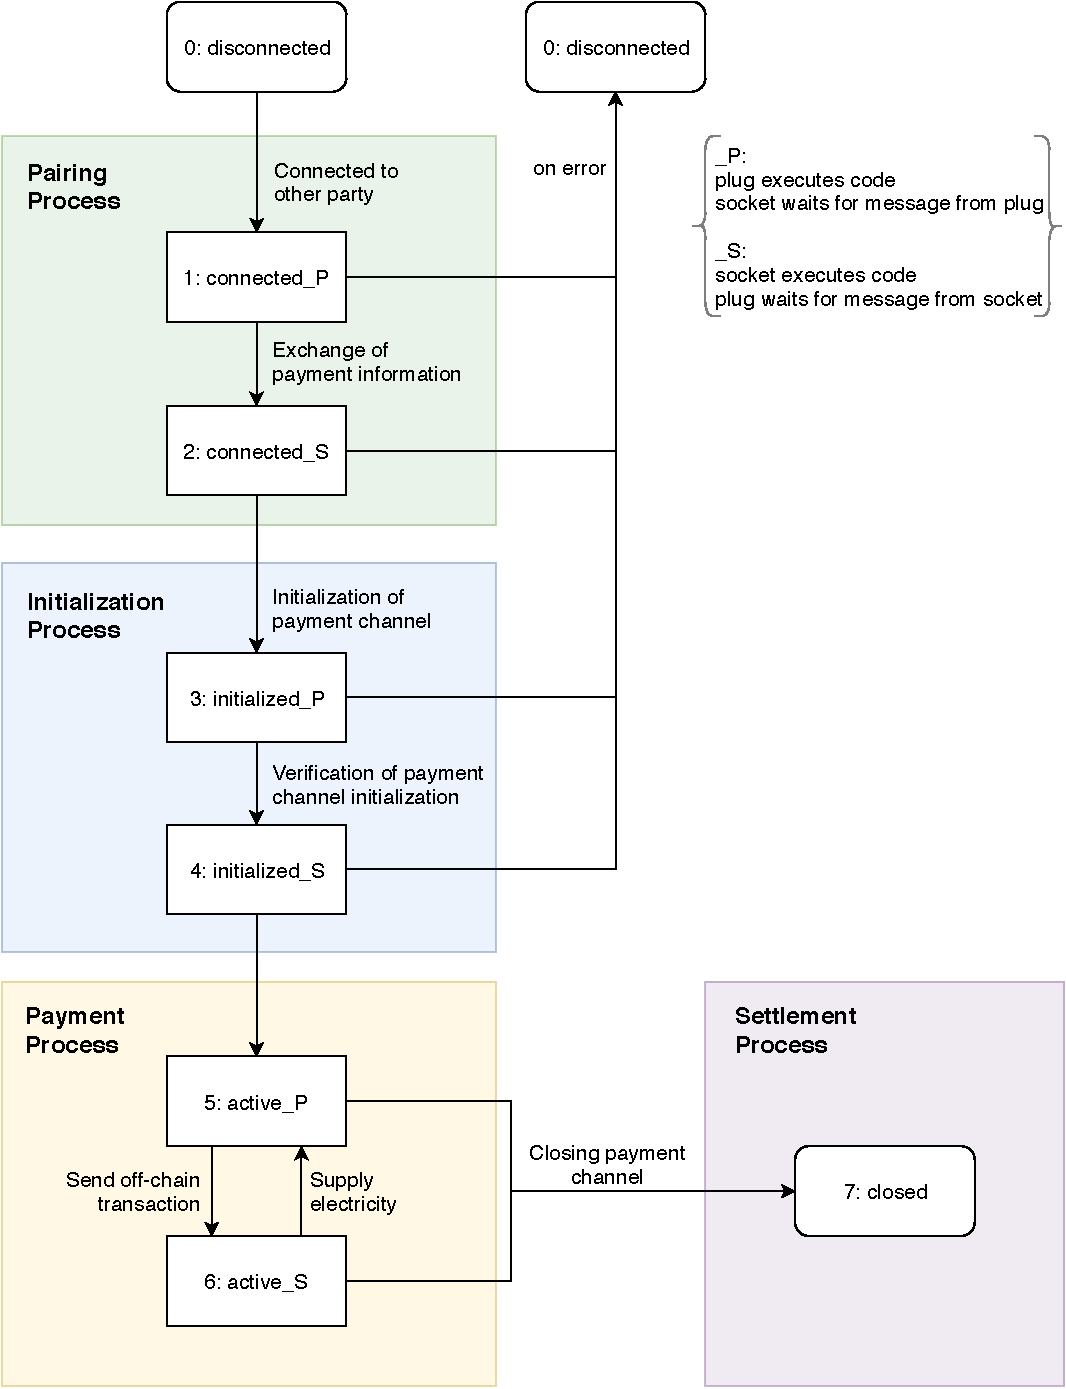
\includegraphics[height=15cm]{img/state_machine.pdf}
    \caption{Concept of the state machine}
    \label{fig:state_machine}
  \end{center}
\end{figure}
According to the different states, different code is executed  – the suffix \textit{\_P} means that the plug is currently executing code and the socket is expecting a message from the plug, \textit{\_S} means the opposite.
\\
During the pairing process, both parties exchange all required payment information with each other.
The payment channel is initialized and all payment information is verified by both parties in the initialization process.
During the third phase, the plug and the socket exchange off-chain transactions for electricity until any party wants to stop the payment process.
Then the settlement process is initialized closing the payment channel and finalizing the transactions on the blockchain.
\\\\\\

\textbf{Pairing Process}\\
The goal of the pairing process is to establish a connection between the customer and the supplier and exchange all necessary payment information.
\\
\begin{figure}[H]
    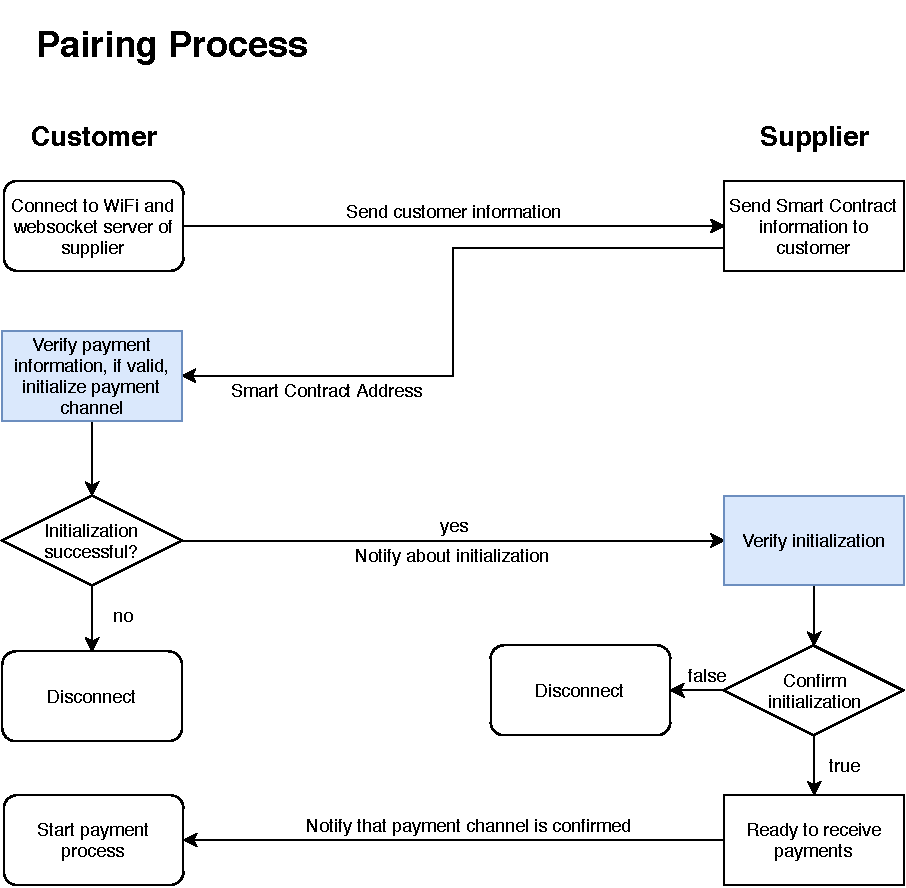
\includegraphics[width=\textwidth]{img/Plug-Socket-pairing_process.pdf}
    \caption{Pairing process}
    \label{fig:pairing_process}
\end{figure}
Both, the customer in form of the plug and the supplier in form of the socket start in the \textit{disconnected} state.
\\\\
As soon as a new customer connects to the socket and wants to purchase electricity, both parties transition to the \textit{connected\_P} state.
The socket now expects the customer information, in this case the Ethereum address, from the plug.
The address is important to know as it will be later used to verify off-chain transactions and whether the payment channel was initialized correctly.
\\\\
When the customer sends the required information, the plug and the socket enter the \textit{connected\_S} state.
The supplier can check the address against white- or blacklists and decide whether to accept payments from this address or not.
If the customer is accepted, the socket transfers the address of the smart contract, as it is required by the customer to fetch the rest of the payment information.
Both parties now enter the initialization process.
\\\\\\
\textbf{Initialization Process}\\
During the initialization process demonstrated in Figure \ref{fig:verification_process} all the necessary payment information is fetched from the smart contract and the payment channel is initialized by the customer.
\\\\
Both parties start in the \textit{initialized\_P} state.
The plug is required to retrieve all relevant payment information which is stored in the smart contract, where it can be easily updated if necessary.
Payment information required for the transaction is the price per second and the payment interval to calculate the value of each off-chain transaction sent.
Optional payment information could be the owner of the smart contract, a minimum deposit value, minimum and maximum charging durations and the expiration date, depending on the implementation.
The plug should also verify that there is no other payment channel currently active.
\\
After the price was fetched from the smart contract, the customer can decide whether to accept the price and continue with the initialization process or to disconnect.
\\
If the price is accepted, an on-chain transaction is signed on the microcontroller and submitted to the Ethereum network.
This transaction calls a function inside the smart contract and initializes the payment channel.
A maximum amount of Ether that the customer is willing to spend during the charging process is passed alongside the smart contract call which will be deposited into the contract.
The customer now has to wait until the transaction was mined.
If the payment channel was initialized correctly, the socket is notified about the initialization and both devices enter the \textit{initialized\_S} state.
\\\\
If the socket can confirm that the payment channel was initialized correctly, it notifies the customer that it is ready to accept off-chain transactions and the payment process begins.
\begin{figure}[H]
    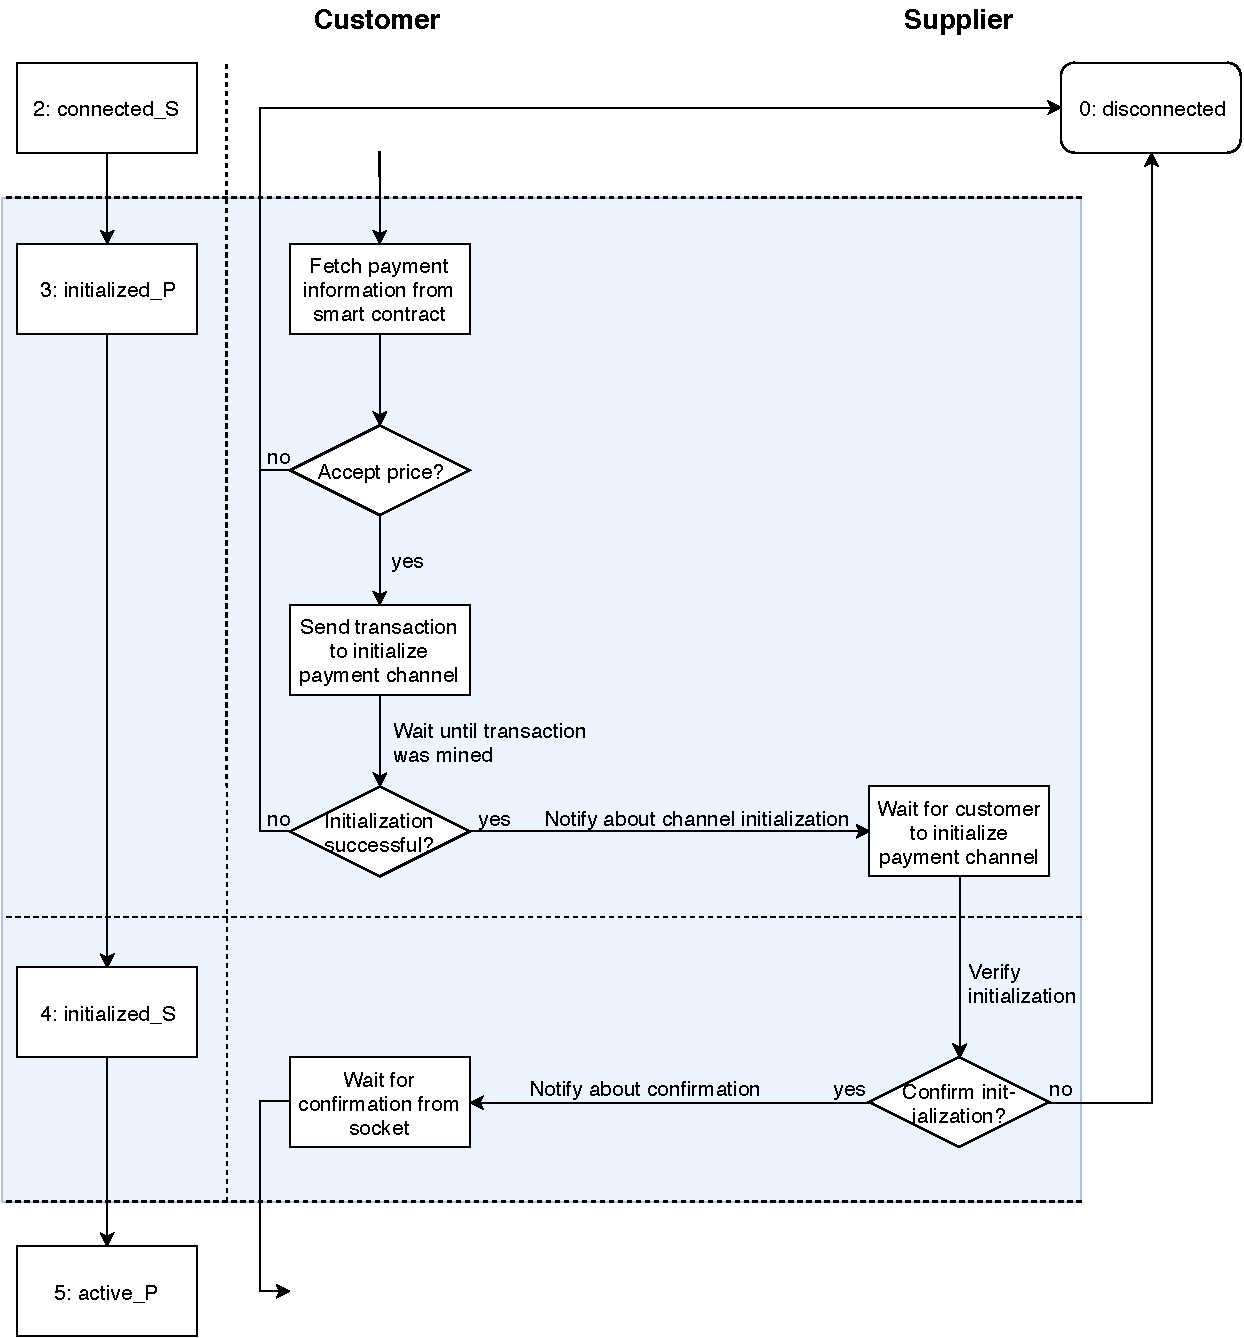
\includegraphics[width=\textwidth]{img/Plug-Socket-verification_process.pdf}
    \caption{Verification process}
    \label{fig:verification_process}
\end{figure}
\leavevmode
\newpage
\textbf{Payment Process}\\
The goal of the payment process is to exchange off-chain transactions for electricity.
\\
\begin{figure}[H]
    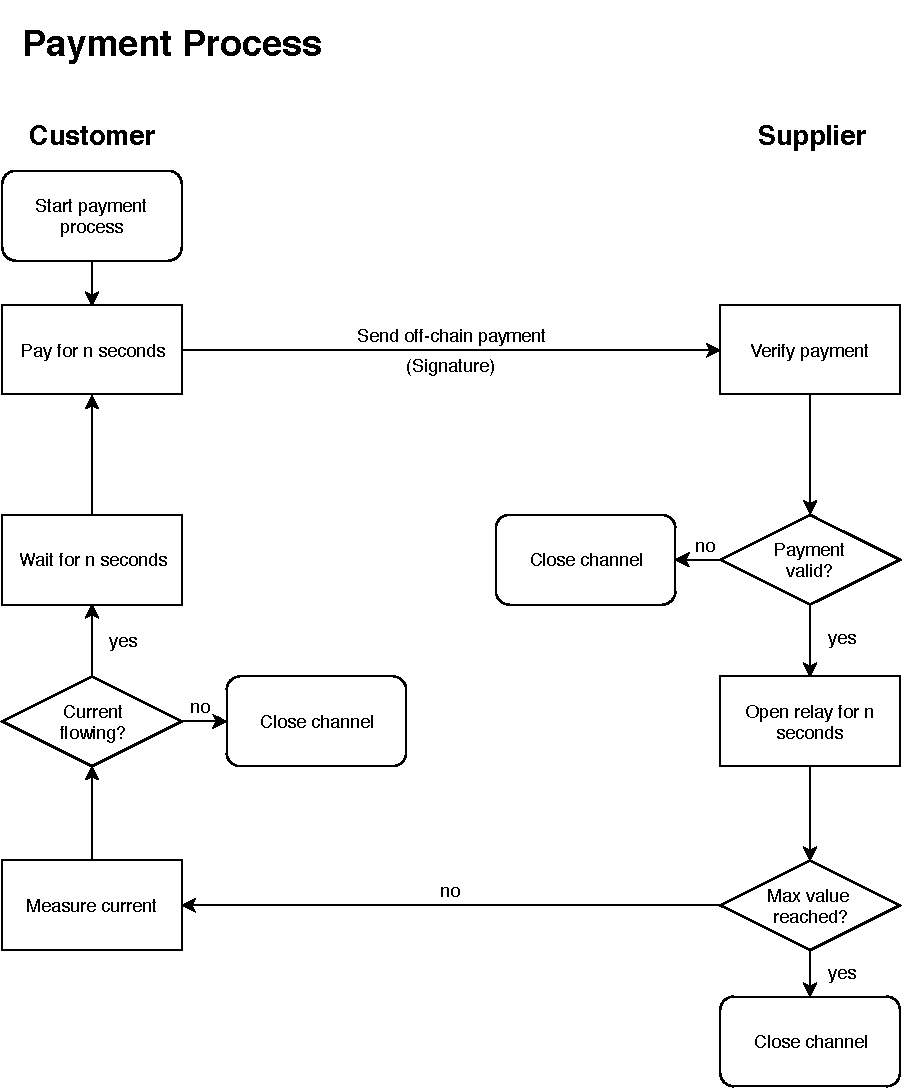
\includegraphics[width=\textwidth]{img/Plug-Socket-payment_process.pdf}
    \caption{Payment process}
    \label{fig:payment_process}
\end{figure}
The payment process starts when the customer sends the first off-chain transaction to the supplier.
As it would be inconvenient for the socket to store and submit hundreds of off-chain transactions, only one signature can be submitted to the smart contract.
With every transaction, the plug increases the value of the off-chain transaction.
Every signature is valid, but it is in the interest of the supplier to submit the latest signature with the highest value.
The value of the transaction is calculated as follows:
\begin{center}
$value = number\_of\_transactions * price\_per\_second * seconds\_between\_transactions$
\end{center}
With the assumed values from Chapter 3 (a total price of 18 \euro{} over a duration of 11 hours) roughly 0.007 \euro{} are transmitted with each off-chain transaction.
With the formula above, this means that the value hashed and signed is 0.007 \euro{} for the first transaction, 0.014 \euro{} for the second, and so on.
As the smart contract operates on ETH and not \euro, the values are converted to Wei first.
\\\\
When the socket receives an off-chain transaction, it should verify that the payment is actually valid.
Both parties keep track of the number of transactions sent and know the price per second, therefore the data that was digitally signed by the customer can be recreated.
Using the data and the signature received from the plug the signer's Ethereum address can be recovered.
It should match the Ethereum address received during the pairing process for the transaction to be valid.
\\
If the off-chain transaction is valid, the microcontroller can close the relay for the specified amount of seconds, supplying the plug with electricity.
\\\\
To ensure that the socket doesn’t deliver more electricity than the plug can pay for, the supplier has to check whether the maximum value, that was deposited into the smart contract, was reached.
If that is the case, the channel is closed, ending the exchange of electricity.
\\\\
After the plug sends a transaction that pays for the specified amount of seconds, it starts measuring the current.
As soon as it is detected, the plug starts a timer and waits an appropriate amount of time to send the next transaction.
For the implementation, a new transaction is sent to the socket when there is 5 seconds of paid electricity left to ensure a steady flow without interruptions.
If the customer paid for electricity, but no current is measured in return, it can immediately interrupt the payment process by closing the payment channel, without losing another payment.
\\\\\\
\textbf{Settlement Process}\\
The settlement process closes the payment channel taking the value of the off-chain transactions and paying out the balances to each participant on the blockchain, finalizing the exchange.
\begin{figure}[H]
  \begin{center}
    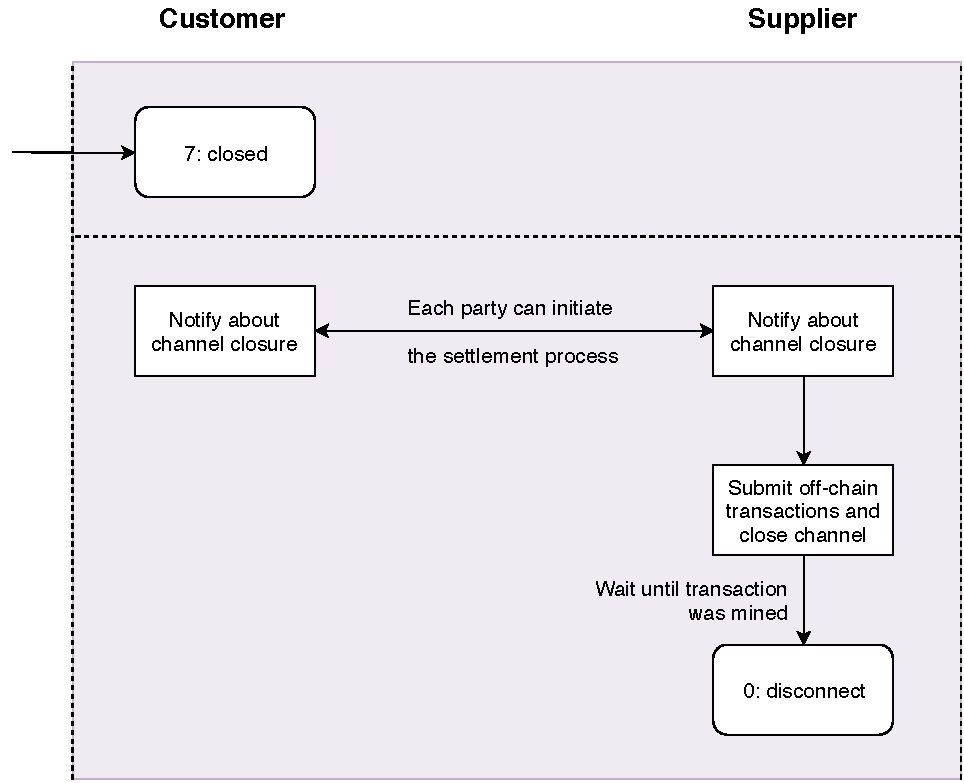
\includegraphics[height=8.6cm]{img/Plug-Socket-settlement_process.pdf}
    \caption{Settlement process}
    \label{fig:settlement_process}
  \end{center}
\end{figure}
As soon as a party wants to stop the payment process, e.g., when the battery of the customer is fully charged or the socket received an invalid signature, it can notify the other party about it.
The socket signs an Ethereum transaction which calls a function inside the smart contract that takes the latest off-chain transaction, which contains the total value spent by the plug up to this point, as an argument.
The smart contract verifies the submitted signature and pays out the amounts accordingly.
\\
The smart contract also protects the customer, as it was mentioned before.
If the supplier fails to submit a valid signature in a certain amount of time and the payment channel expires, the deposited amount can be withdrawn again.
\\
\subsection{Transactions}
During the initialization, payment and settlement process transactions have to be sent by the plug and socket.
This section will go into detail on how transactions were implemented for this thesis.
\\\\
When researching existing implementations of the generation of on-chain transactions for the Ethereum network on a microcontroller level, it was discovered that these implementations are far from production ready, as opposed to implementations with high level programming languages.
In an effort to find existing code that could be used as a foundation for the implementation some utility libraries were found, but many of them were not compatible with the microcontroller and the ones that were, often had to have issues fixed or additional functions implemented.
\\\\
Payment channels and off-chain transactions were implemented in this bachelor thesis as well.
They are a subset of state channels, which currently are a heavily researched topic on their own, therefore no standard exists that could be followed for the implementation.
As far as exploratory research went, every state channel implementation was still under development and not a single implementation of a payment channel on an embedded level could be found\cite{state-channels}.
Therefore an entire concept for the payment channel had to be developed, that could run on microcontrollers.
\\\\
The process of sending an on-chain transaction can be broken down into the following steps: 
\begin{enumerate}
    \item Gather data
    \item Encode data
    \item Hash data
    \item Sign hash
    \item Submit signature
\end{enumerate}
Off-chain transactions were implemented in a way to mimic the functionality of on-chain transactions.
The following paragraphs will go into detail of the implementation of on- and off-chain transactions, why certain design choices were made and which challenges were faced.
\\\\\\
\textbf{1. Gather Data}\\
The following information is necessary to send an on-chain transaction on the Ethereum blockchain:
\begin{enumerate}
  \item \textit{to}: Receiving address of the transaction.
  \item \textit{value}: Value of the transaction in Wei.
  \item \textit{data}: Hexadecimal data can be passed with the transaction.
  When sending a transaction to a smart contract, the data is used to define which function is called and to pass arguments.
  The first four bytes are the function identifier followed by the function arguments which are encoded according to the "ABI specification"\cite{abi-encoding}.
  As the signature, which is a dynamic byte array, is passed to the smart contract alongside other variables, the encoding according to the specification had to be implemented.
  \item \textit{nonce}: The nonce is important, as it protects a user against replay attacks and guarantees that transactions are executed in the correct order.
  The nonce starts at zero and increments by one after a transaction was sent.
  This means that transactions, where the nonce is less than the total amount of transactions sent by the account, are rejected by the Ethereum network.
  Without the nonce an attacker could resubmit a transaction, that was already mined, over and over again to drain the balance of a victim.
  \item \textit{gas price}: The fee of a transaction that gets paid out to a miner in Wei.
  The higher the fee, the faster the transaction will be mined.
  The Rinkeby testnet uses a \abbr{Proof of Authority}{PoA} mining algorithm, which only allows a few accounts to act as miners, as in a test environment without monetary incentives, stability is more important than decentralization.
  Therefore there are no competing miners and high transaction fees are not relevant.
  A transaction with a gas price of 1~GWei will be usually included in the next block resulting in a confirmation time of less than 15 seconds.
  On the mainnet the gas price should be checked carefully, so the transaction is mined in a reasonable amount of time to not interfere with user experience.
  \item \textit{gas limit}: The gas limit specifies how much code can be executed with a transaction.
  The base limit of any transaction, whether it is a smart contract call or not, is 21,000 gas – it covers the storage of the transaction on the blockchain as well as the elliptic curve operation to recover the sender of the transaction\cite{design-rationale}.
  Each additional computational step costs more gas, e.g., an addition (opcode: ADD) costs 3 gas, loading a variable from storage (opcode: SLOAD) costs 200 gas and even goes as far as 20,000 gas if a storage value (variable stored on the blockchain) is set from zero to non-zero.
  As it can be seen, storing data on the blockchain is one of the most expensive operations to discourage storing vast amounts of information on-chain.
  If the gas limit is set too low and there is not enough gas to finish the smart contract execution, the transaction is unsuccessful and reverts any changes made.
  If the limit was set too high, any unused gas is refunded to the sender.
  Thus, when implementing smart contract calls on the microcontroller, it is important to provide enough gas for all computations.
  The total transaction fee is calculated by multiplying the gas price with the gas limit.
  \item \textit{chain ID}: Each Ethereum blockchain has a unique chain ID to differentiate between different chains.
  For example the mainnet uses the ID 1 and the Rinkeby testnet uses the ID 4.
  With the Ethereum Improvement Proposal 155 (EIP-155)\cite{eip-155} the chain ID should be included into a transaction to prevent so-called cross chain replay attacks, where a transaction on one Ethereum chain can be resubmitted to another Ethereum chain.
\end{enumerate}
\leavevmode
\\
Although the functionality of off-chain transactions mimic on-chain transactions, not every parameter listed above is required.
Because the payment channel was implemented between two parties only, the \textit{to} parameter can be left out.
The value, as demonstrated in the previous chapter, is defined as the total value spent up to a specific point in Wei and is included in the off-chain transaction.
There is no need to pass any data with the off-chain transactions, therefore no data is included.
No transaction fees are paid either, so the gas limit and gas price can be dropped from the off-chain transaction.
A nonce is mandatory to protect the customer. Without it, a supplier could just resubmit an off-chain transaction with a higher value from a previous exchange, stealing money from the customer. The smart contract keeps track of the nonce of each customer and needs to be fetched by both parties during the initialization process.
Although the \textit{chain ID} is not required to be included, a similar kind of attack can be conducted across different smart contracts.
If every socket has its own smart contract, an off-chain transaction with a higher value originally submitted on one smart contract, can be wrongfully resubmitted for a different exchange on another smart contract.
Therefore, the address of the smart contract managing the payment channel is included inside the off-chain transaction.
\\\\\\
\textbf{2. Encode Data}\\
On-chain transactions are encoded with the \abbr{Recursive Length Prefix}{RLP}\cite{ethereum-yellow-paper}.
Before the data listed above is hashed, it is converted into hexadecimal and therefore byte-arrays.
The benefit of RLP encoding is that parameters of variable length are encoded in a way that all parameters can be extracted from the resulting byte array in the end.
This is mandatory, so miners can extract the required data from the encoded byte array to fulfill the transaction.
RLP was especially designed for Ethereum to efficiently encode these values with the following rules: 
\begin{itemize}
  \item If a single byte is in the range of 0x00 and 0x7f, the byte is its own encoding.
  \item If a byte array is 0 to 55 bytes long, the byte array is prefixed with a single byte with the value 0x80 plus the length of the byte array.
  \item If a byte array is longer than 55 bytes, it is encoded by a first byte that has the value 0xf7 plus the length of the length prefix of the byte array, followed by the bytes describing the length of the byte array and finally the byte array itself.
  \item A list of byte arrays can be encoded as well, as it is required for the transaction data.
  All items are encoded individually first and then encoded again as a total byte array.
  This allows to encode data, no matter how nested the information is.
\end{itemize}
For the implementation, code from a RLP C++ library was used, which was written by Takahiro Okada\cite{rlp-lib}.
The following changes had to be made to the library so it could be used for the implementation.
\begin{itemize}
  \item The library had to be rewritten, to implement encoding of transactions into one utility library and to make it compatible with the microcontroller.
  \item The library now supports the EIP-155\cite{eip-155} when encoding transactions with the chain ID.
  \item A wrong calculation was fixed that would incorrectly encode byte arrays longer than 55 bytes.
  \item The memory allocation of the library had to be adjusted, as it did not allocate enough memory to handle all data that needed to be encoded for the transactions.
\end{itemize}
\leavevmode
\\
The smart contract validates an off-chain transaction by recreating the signed data and using it to recover the signers address from the signature.
As the nonce and the contract address are already stored inside the smart contract, only the value and the signature have to be passed to the smart contract function.
The Solidity smart contract programming language uses so-called encoding in packed mode before hashing as a standard\cite{packed-spec}:
\\
\begin{lstlisting}[language=Solidity, numbers=none]
abi.encodePacked(
  _value,
  contractAddress,
  customerNonce
)
\end{lstlisting}
\leavevmode
\newpage
To ensure consistency, the same encoding had to be implemented on the microcontrollers with the following rules:
\begin{itemize}
  \item all variables are converted to bytes and concatenated together
  \item "types shorter than 32 bytes are neither zero padded nor sign extended"\cite{packed-spec}
  \item "dynamic types are encoded in-place and without the length"\cite{packed-spec}
\end{itemize}
\leavevmode
\\\\
\textbf{3. Hash data}\\
The encoded data of both, on- and off-chain transactions, is hashed using the Keccak-256 hashing algorithm.
This algorithm is almost identical with the official SHA-3 implementation, but Ethereum uses Keccak-256 instead, which was "the winning entry to the SHA-3 contest"\cite{ethereum-yellow-paper}.
\\\\
Before signing a signature that is used on the Ethereum blockchain, e.g., an off-chain transaction, it is recommended that the data is prefixed with an Ethereum specific prefix\cite{prefix}.
The prefix makes the signature recognizable as an Ethereum specific signature and protects users from attackers letting them unknowingly sign a transaction, instead of a message.

The encoded data is hashed, then prefixed according to the following rules:
\\
"\textbackslash x19Ethereum Signed Message:\textbackslash n" + len(message) + message
\\
As a 256 bit hash is the message that is signed, the length of the prefix is always 32 bytes.
The prefixed message is then hashed again:
\\
\begin{lstlisting}[language=Solidity, numbers=none]
bytes32 message = keccak256(
  abi.encodePacked(
    value,
    contractAddress,
    customerNonce
  )
);

bytes32 prefixedMessage = keccak256(
  abi.encodePacked(
    "\x19Ethereum Signed Message:\n32",
    message
  )
);
\end{lstlisting}
The plug mirrors the smart contract implementation demonstrated above during the generation of off-chain transactions.
It needs to produce the same hash for the same input data as the smart contract to make it verifiable for the closure of the payment channel.
\newpage
\textbf{4. Sign data}\\
Although Ethereum relies on ECDSA elliptic curve signatures, there are some additional rules and features that differ the signature process from its standard implementation:
\begin{itemize}
  \item It takes up to two guesses to recover the public key / address from the $r$ \& $s$ values of an ECDSA signature.
  Therefore, a third value $v$, also called the \textit{recovery ID} is calculated, that enables the immediate extraction of a public key from a signature.
  According to the Ethereum yellow paper\cite{ethereum-yellow-paper} "the recovery identifier is a 1 byte value specifying the parity and finiteness of the coordinates of the curve point for which r is the x-value".
  The recovery ID is determined during the signature process by looking at the y value on the elliptic curve with the following formula:
  \\
  $v = 27 + (y \% 2)$
  \\
  i.e., if y is even the recovery ID equals to 27, if it is odd, it equals to 28.
  The formula is used for signatures of all kinds.
  With the aforementioned EIP-155, optionally the following formula can be used for on-chain transactions, securing them against cross-chain replay attacks:
  \\
  $v = chain\_id * 2 + 35 + (y \% 2)$
  \\
  This means that for transactions on the Rinkeby network, the recovery ID is either 43 or 44.
  For the generation of off-chain transactions the first and for on-chain transactions the second formula was implemented on the microcontrollers.
  \item According to the Ethereum yellow paper\cite{ethereum-yellow-paper} the $s$ part of the signature has to be less or equal than half of the numeric value of the elliptic curve $n$.
\end{itemize}
As a foundation, a standard implementation of the ECDSA algorithm\cite{micro-ecc} was used.
Both additional features of the Ethereum specific signatures had to be implemented extending the library.
\\\\\\
\textbf{5. Submit signature}\\
To submit an on-chain transaction, the transaction data and the signature has to be RLP encoded again.
The resulting byte array can then be submitted to the Ethereum network by sending the transaction to the node.
\\\\
As previously mentioned, both the plug and the socket keep track of all transaction data themselves.
Therefore, when the plug is paying for electricity with an off-chain transaction, it simply sends the signature to the socket.
\\\\\\
\textbf{Additional challenges}\\
Smart contracts mainly work with 256 bit unsigned integers for numbers, but most microcontrollers are not capable of working with integers this big.
When fetching a \textit{uint256} value from a smart contract, the value returns as a hexadecimal string from the node.
The largest fixed width integer type \textit{uint64\_t} or \textit{unsigned long long} can only store 64 bits of data which equals roughly 18.44 ETH.
If the value exceeds exceeds 64 bit, parsing, storing and calculating with the value becomes a lot more challenging, as the data has to be processed as a byte array.
\\\\
As all the communication with the Ethereum blockchain is processed through the node and http requests, all data is mostly handled as hexadecimal represented by char arrays.
These use more space than byte arrays.
During the entire process of generating on-chain transactions, the data for the smart contract call has to be encoded, then encoded with the rest of the transaction data, hashed, signed and the resulting signature has to be encoded with the transaction data again.
The generated transaction then has to be put into a JSON http request body and the response that returns from the node has to be JSON parsed to receive required data.
This generates a lot of data mainly in the form of char arrays which can get long, depending on the arguments passed to a smart contract.
On an embedded platform with limited memory a lot of optimization and memory management is required to successfully generate a transaction.
\\\\
\subsection{Smart Contract}
Security is extraordinarily important for smart contract development, as possibly large sums of money are handled and the code is immutable, and can’t be changed once the smart contract has been deployed to the Ethereum network.
This section will go over the smart contract implementation, some security best practices and design choices.
The entire source code can be found within the appendix, listings \ref{lis:safemath} \& \ref{lis:pc_sc}.
\\\\
The smart contract was designed in a way that only one contract is responsible for one socket which can only handle one payment at the time.
One of the most important rules for smart contract development is to keep the code as simple as possible.
Adding complexity only increases the risk of a critical issue.
When the customer initializes the payment channel, a maximum transaction value is deposited which is kept inside the smart contract until the channel is closed or expires.
Additionally, the address of the customer is stored inside the smart contract as a global variable which will be used to verify the off-chain transactions:
\begin{lstlisting}[language=Solidity, numbers=none]
// set channel customer to the address of the caller of the transaction
channelCustomer = msg.sender;
\end{lstlisting}
\leavevmode
\\
The channel can be timed out by any participant on the network after the expiration date has been reached, returning the deposited funds to the customer.
The function to close the channel can only be called by the supplier.
The total transaction value and the signature of the final off-chain transaction is passed to the function as an argument.
From the three values inside the off-chain transaction, the transaction data is regenerated.
The nonce and the address of the smart contract cannot be forged, as these values are not passed by the supplier.
Instead, they are taken directly from the storage of the smart contract itself.
The smart contract repeats the same steps to generate the transaction data as the plug – the data is hashed and prefixed with the Ethereum specific prefix:
\\
\begin{lstlisting}[language=Solidity, numbers=none]
bytes32 message = keccak256(
  abi.encodePacked(
    // value passed as an argument
    _value,
    // variable to receive the smart contract address
    address(this),
    // gets the nonce of the current channel customer
    customerNonces[channelCustomer]
  )
);

bytes32 prefixedMessage = keccak256(
  abi.encodePacked(
    "\x19Ethereum Signed Message:\n32",
    message
  )
);
\end{lstlisting}
\leavevmode
\\
The computed \textit{prefixedMessage} should result in the same data that the customer used to sign the off-chain transaction.
Solidity offers a function to recover the address of the signer, if provided with the signed data and the signature.
\\
\begin{lstlisting}[language=Solidity, numbers=none]
return ecrecover(prefixedMessage, v, r, s) == channelCustomer;
\end{lstlisting}
\leavevmode
\\
The function returns true if the recovered address matches the current payment channel customer.
The verification of the off-chain transaction is tamper proof.
If the supplier tried to provide a false value with the signature, the recreation of the data would result in data that the customer did not sign.
Therefore, the \textit{ecrecover} function would return an address that does not match the current channel customer.
Only the correct data both parties agreed to can be used to close the payment channel.
\\\\
If the signature was valid, the nonce of the customer increments by one, making all off-chain transactions up to this point invalid.
Then the transaction value is paid out to the supplier and the rest is refunded to the customer, closing the payment channel.
\newpage
\subsubsection{Best practices}
The smart contract implements the so-called pull over push method\cite{best-practice}.
When closing the payment channel, the according transaction values could be immediately paid out to the customer and the supplier.
An attacker could write a smart contract that would initialize a payment channel and would always revert the transaction when it received Ether during the settlement.
In this case the payment channel would be locked forever, as the customers balance could be never paid out.
Instead, a balance variable is used, from which each party can withdraw their share without the risk of blocking the smart contract.
\\\\
Solidity has no built in checks for integer under- and overflows, which can become a major security issue, especially when dealing with balances, allowing an attacker to drain a smart contract.
A so-called SafeMath library, as the one found under Listing \ref{lis:safemath} can help in preventing integer under- and overflows.
\\\\
Another security concern that comes up when withdrawing Ether from balances is the reentrancy attack.
In traditional programming, an amount would be paid out and upon success, the balance would be adjusted to reflect the new balance.
In smart contract programming this practice resulted in a hack where an attacker recursively withdrew the balance from a smart contract, resulting in theft of over 3.6 million ETH, which is worth 792 million \euro{} at the time of writing\cite{dao-hack}.
Therefore, it is very important to set the new balance before transferring Ether.
If the transfer fails, the entire smart contract call is reverted, so the new balance only comes into effect if the transaction was successful.
\newpage
\clearpage
\section{Conclusion}
The goal of this thesis was to examine whether M2M payments could be implemented on a microcontroller level and which payment method was suited best for this task.
A concept of an electrical plug and an electrical socket was developed, which exchange electricity for monetary value.
This worked out concept was successfully implemented on embedded devices.
\\\\
An underlying payment system was developed to enable fast and secure transfers of monetary value between two participants.
The system uses the Ethereum blockchain to initialize and settle a payment channel, which enables instant and feeless transactions between parties inside this channel.
The transactions are secured through digital signatures and the smart contract acts as a trustee managing the monetary value while protecting both parties from fraud and minimizing the risk of theft dramatically.
The payment system enables a true P2P market, allowing everyone to become a charging station provider and to securely sell electricity to electric car owners.
As there is no need for a third party as a middleman that oversees the transaction, the total transaction fees for a charging process of any length and value should average at less than 0.10 \euro{} at the time of writing.
This bachelor thesis can not only be used for this specific concept, but many different P2P business models can be developed using the payment channel as a base as well.
\\\\
This implementation is most likely the first implementation of a payment channel on an embedded platform, as far as research went.
For Ethereum specific functionalities, e.g., signatures and encoding that were especially created for the blockchain technology, libraries exist in high level programming languages, but had to be implemented on embedded devices for this purpose.
Additionally, many computational steps and memory allocation had to be optimized to make the payment system work on microcontrollers.
This means that the code that was written for this bachelor thesis can be used in the future not only for payment channels, but as the groundwork for basically any communication between an embedded device and the Ethereum blockchain and smart contracts.
\\\\
\subsection{Outlook}
As cryptocurrencies are still in their infancies, most of the development is still ahead and nobody can imagine what they will look like in 10 years.
Similarly, when the internet was in its infancy, no-one imagined that something like Facebook could even exist.
The technology will scale to process more transactions at even lower fees and will be steadily integrated more and more into our daily lives.
For example, in its latest flagship, the Galaxy S10, Samsung included an Ethereum and Bitcoin wallet, meaning that millions of people are now able to transact with cryptocurrencies securely without any big entry barriers.
\\\\
Eventually, the price of cryptocurrencies will stabilize, but until that happens, some suggestions for future work that can build upon this thesis are proposed.
Currently, the microcontrollers are communicating with each other over a WiFi connection and WebSockets and the plug has to be powered separately to function.
An implementation that would improve upon this, would have the socket and the plug communicate over PLC, i.e., over the electricity that is transmitted.
Before the actual electricity delivery, the socket could limit the output so that the microcontroller of the plug can be powered and communicated with, without the need for an external energy source.
Another interesting topic would be to implement the payment system with other cryptocurrencies, such as IOTA or Nano to analyze the key strengths and weaknesses of the different payment methods.
As fast as the crypto-ecosystem develops, there could be new cryptocurrencies in a few months that couldn’t even be considered during this thesis.
In about a year at the time of writing, Ethereum plans to upgrade to a new blockchain, also called Ethereum 2.0\cite{eth-2} which will implement a new mining algorithm and lots of different scaling solutions.
This might bring potential new ways to implement an even more efficient payment system.
\newpage
\clearpage
%%%%%%%%%%%%%%%%%%%%%%%%%%%%%%%%%}}}%
% Appendix                          %
%%%%%%%%%%%%%%%%%%%%%%%%%%%%%%%%%{{{%
\newpage
\clearpage

%clear headers
\fancyhead{}
\fancyfoot{}
\fancyfoot[CO, CE] {\thepage}

%\section{Appendix}

%%%%%%%%%%%%%%%% >INSERT YOUR APPENDIX HERE>
\section{Appendix}
\label{sec:appendix}
\subsection{Setup Instructions}
This section will focus on the technical setup of the hardware components of a functioning prototype and the installation and setup of all required software.
\\
\subsubsection{Socket}
The Sonoff S20 smart socket was used for the technical implementation of the concept.
A microcontroller is automatically powered by the socket it is plugged into.
The S20 also has a WiFi module and a relay, which can be switched on and off by the microcontroller.
The microcontroller can be reprogrammed via a serial port.
To program the Sonoff S20 the device has to be opened, revealing the logic board with the relay and the serial port.
\\
\begin{figure}[H]
    \includegraphics[width=\textwidth]{img/S20_open.png}
    \caption{Sonoff S20}
    \label{fig:S20}
\end{figure}
\newpage
To program the microcontroller with a computer a FTDI USB to serial converter is used.
The converter has to be plugged into the S20 as follows:
\\
\begin{center}
    \begin{tabular} { |c|c| }
        \hline
        FTDI Converter & Sonoff S20 \\
        \hline\hline
        GND & GND \\
        \hline
        TX & RX \\
        \hline
        RX & TX \\
        \hline
        3.3V & 3.3V \\
        \hline
    \end{tabular}
    \captionof{table}{Connection between serial converter and microcontroller pins}
    \label{tab:ftdi}
\end{center}
\leavevmode
\\
It's important to notice that the FTDI converter must operate at 3.3V entirely.
Caution: some converters only switch the TX and RX pin to 3.3V while the VCC remains at 5V.
This can fry the internals of the S20.
To program the microcontroller, the button has to be pressed before plugging the pins into the serial port to put it in programming mode.
After the pins have been inserted, the button can be released shortly after.
\\
\begin{figure}[H]
    \includegraphics[width=\textwidth]{img/serial_port.png}
    \caption{Serial ports of the Sonoff S20}
    \label{fig:S20_serial}
\end{figure}
\newpage
Both, the socket and the plug, are programmed using the Arduino IDE.
The following steps need to be followed to install the ESP8266 Board, which the S20 is based on:

\begin{itemize}
    \item Inside the Arduino IDE open "Preferences"
    \item Enter \url{http://arduino.esp8266.com/stable/package_esp8266com_index.json} under "Additional Boards Manager URLs"
    \item Open Tools $\rightarrow$ Board $\rightarrow$ Boards Manager
    \item Search and install "esp8266" by "ESP8266 Community"
\end{itemize}

After connecting the FTDI converter to the computer, it should appear under Tools $\rightarrow$ Port.
To successfully flash code to the S20 the following settings have to be set:

\begin{itemize}
    \item \textit{Board}: "Generic ESP8266 Module"
    \item \textit{CPU Frequency}: "80 MHz"
    \item \textit{Flash Size}: "1M (no SPIFFS)"
\end{itemize}
\leavevmode
\subsubsection{Plug}
The device to control the measurement of current in the plug and handle the communication with the socket is the Heltec WiFi Kit 8, which is based on an ESP8266 as well and has a 0.91 inch OLED display.
\\
\begin{figure}[H]
    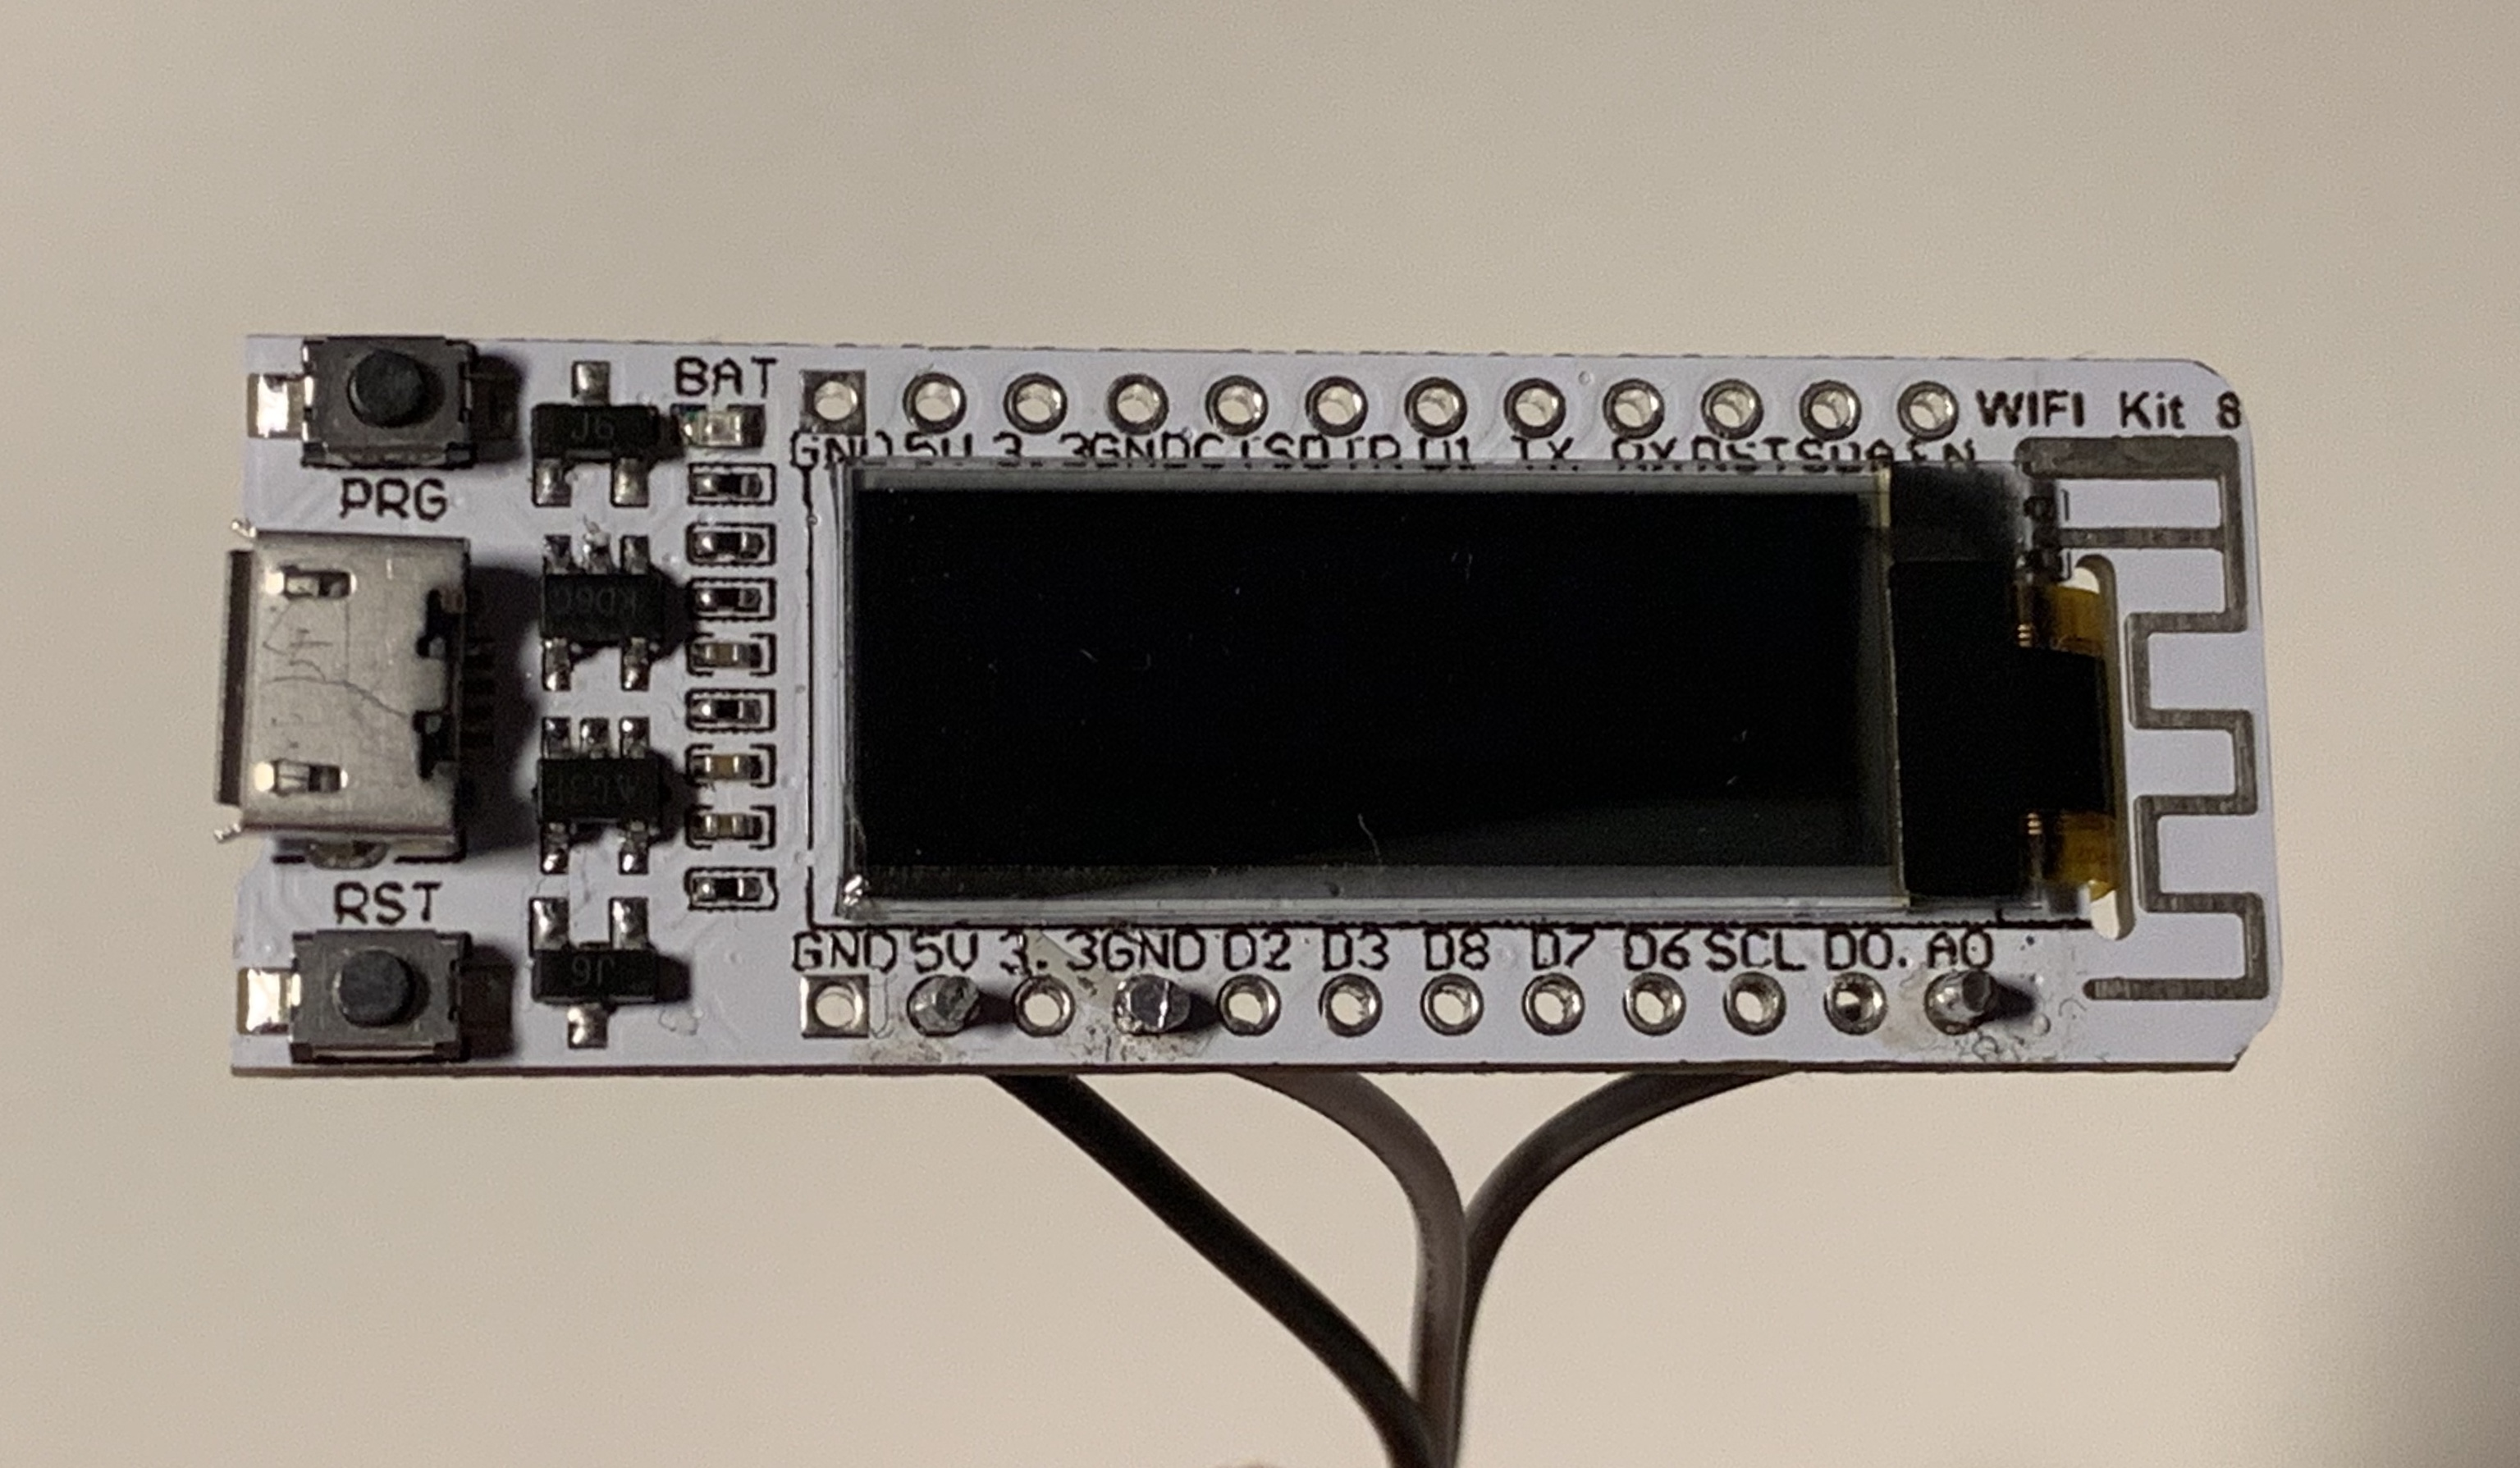
\includegraphics[width=\textwidth]{img/heltec.jpg}
    \caption{Heltec WiFi Kit 8}
    \label{fig:heltec}
\end{figure}

The ACS712 20A current meter is used to measure the current.
It's hall effect-based and provides galvanic isolation up to a minimum of 2.1 kV (RMS)\cite{acs712}.
To connect the current meter, a part of the hot wire leading to the plug has to be cut and stripped.
Both ends have to be inserted into the screw terminal of the ACS712.
The current from the plug is now redirected underneath the hall sensor.
\\
\begin{figure}[H]
    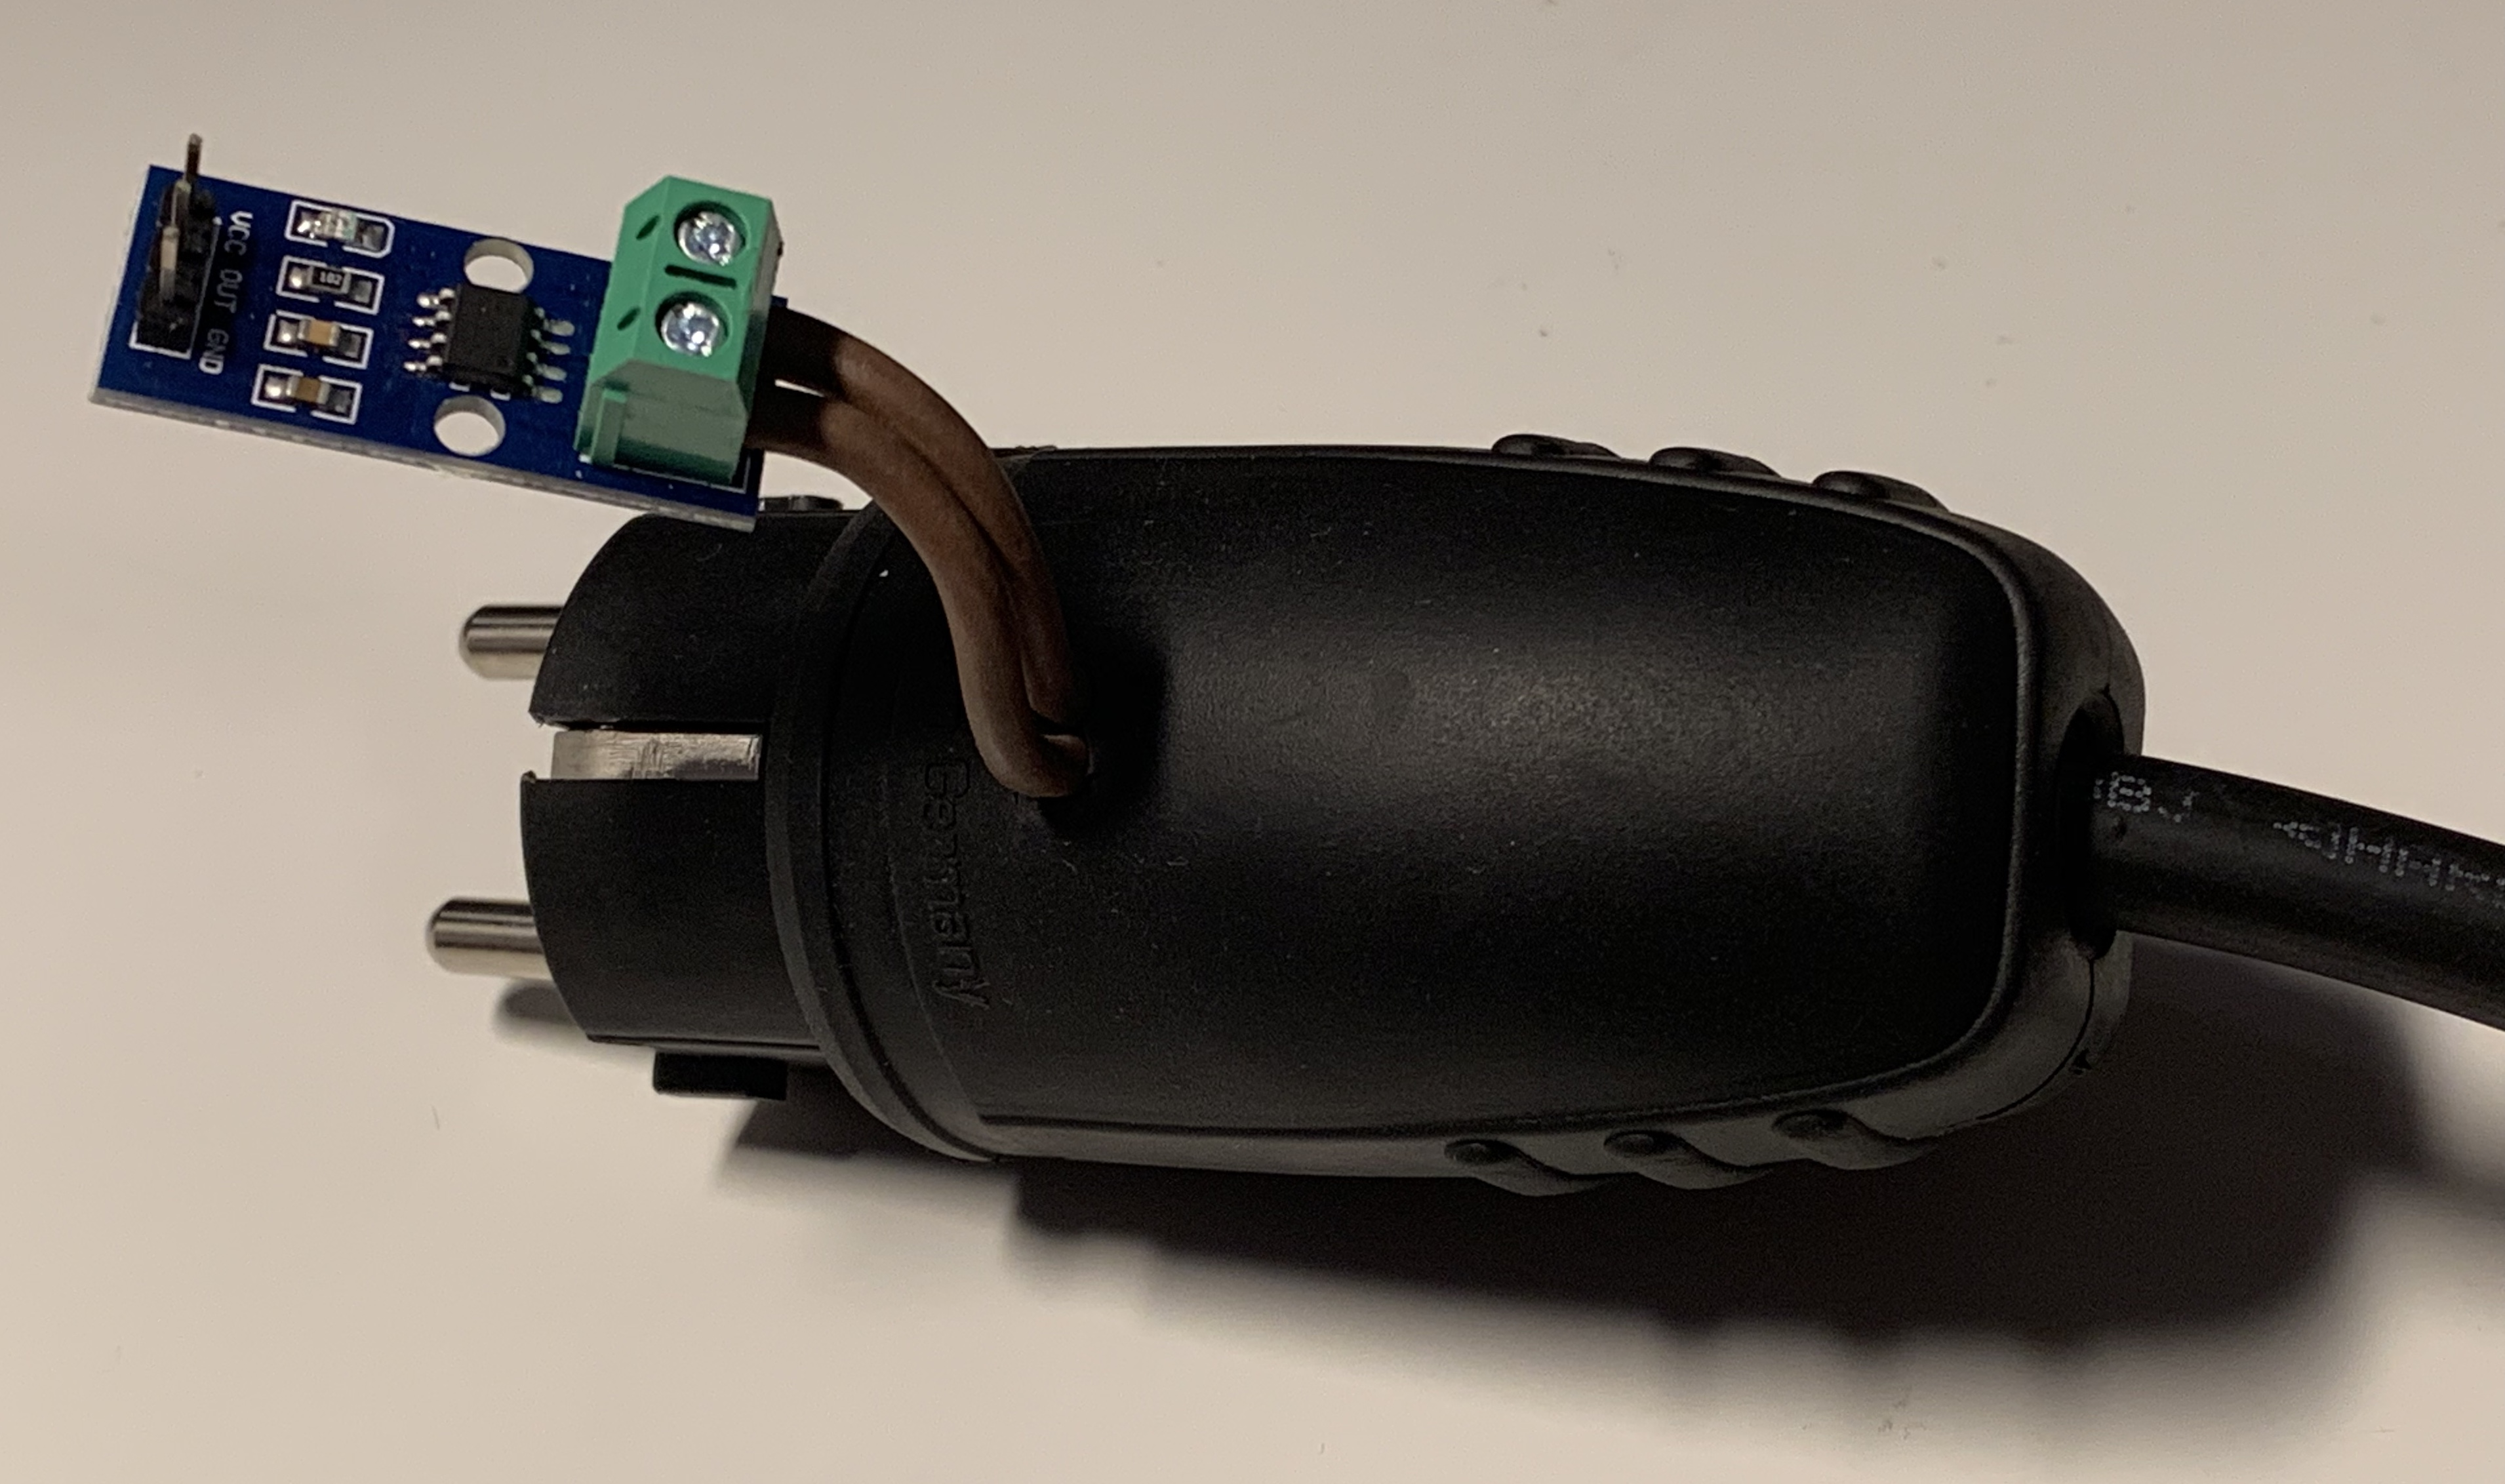
\includegraphics[width=\textwidth]{img/acs712.jpg}
    \caption{ACS712 current meter connected to plug}
    \label{fig:acs712}
\end{figure}

The pins of the current meter have to be soldered to the Heltec board as follows:
\\
\begin{center}
    \begin{tabular} { |c|c| }
        \hline
        ACS712 & Heltec WiFi Kit 8 \\
        \hline\hline
        VCC & 5V \\
        \hline
        OUT & A0 \\
        \hline
        GND & GND \\
        \hline
    \end{tabular}
    \captionof{table}{Connection between current meter and microcontroller pins}
    \label{tab:currentmeter}
\end{center}
\leavevmode
\\
To program the Heltec WiFi Kit 8, USB to UART drivers need to be installed first.
The download link can be found under "References"\cite{vcp-drivers}.
Next, if the ESP8266 was not installed inside the Arduino IDE yet, the instructions found in the subsection above can be used to install the board.
\\
After a successful driver installation, the board should be found under Tools $\rightarrow$ Port when the device is connected to the computer.
\newpage
The following settings are required to ensure a successful flash of the Heltec WiFi Kit:

\begin{itemize}
    \item \textit{Board}: "NodeMCU 1.0 (ESP-12E Module)"
    \item \textit{CPU Frequency}: "160 MHz"
    \item \textit{Flash Size}: "4M (3M SPIFFS)"
\end{itemize}
\leavevmode
\subsubsection{Libraries}
The prototype relies on some external libraries that have to be installed additionally:
\\\\
\textbf{Display}\\
To use the display of the Heltec WiFi Kit a special library needs to be installed.
Inside the Arduino IDE, under Sketch $\rightarrow$ Include Library $\rightarrow$ Manage Library search for and install the "U8g2" library by "oliver".
\\\\
\textbf{WebSocket server}\\
The communication between the plug and the socket relies on WebSockets.
Download the library as a zip file from the git repository\cite{websockets}.
\\
Install it via Sketch $\rightarrow$ Include Library $\rightarrow$ Add .ZIP Library.
\\\\
\textbf{Keccak-256 Library}\\
The implementation relies on a library that was written by Aleksey Kravchenko and was found in the source code of the firefly DIY hardware wallet\cite{keccak-source}.
This library is included with the source code.
\\\\
\textbf{ECDSA Library}\\
Ethereum relies on the Elliptic Curve Digital Signature Algorithm, although there are some differences to the standard implementation of that algorithm.
The zip library is provided with the source code of this prototype and extends the "micro-ecc" library by Kenneth MacKay\cite{micro-ecc}.
\\
\subsubsection{Node}
A server is mandatory to act as a gateway to the Ethereum blockchain.
Geth is the official "Golang implementation of the Ethereum protocol"\cite{geth} and is used to run a full node.
After the installation it will be used to send transactions and make smart contract calls.
\\\\
A \abbr{Virtual Private Server}{VPS} was used for this implementation running Ubuntu 18.04. The server has a six core CPU, 16 GB of RAM, 400GB SSD and 400 MBit/s unlimited traffic.
The following instructions can be used to install the program under Ubuntu.
For other environments the link to the instructions can be found under "References"\cite{geth-instructions}.
To install geth add the repository first:
\begin{lstlisting}[language=bash, numbers=none]
  $ sudo add-apt-repository -y ppa:ethereum/ethereum
\end{lstlisting}

Next, install geth:
\begin{lstlisting}[language=bash, numbers=none]
  $ sudo apt-get update
  $ sudo apt-get install ethereum
\end{lstlisting}
\leavevmode
\\
To interact with the Ethereum blockchain the entire chain history has to be downloaded first.
This can take up to 40 GB of disk space and will take several hours of synchronizing.
Geth will be started via this console command:
\begin{lstlisting}[language=bash, showstringspaces=false, numbers=none]
  $ geth console --rinkeby --rpc --rpcapi="db,eth,net,web3,
  personal,txpool" --rpcaddr X.X.X.X --rpcport 8545 --cache=2048
\end{lstlisting}

The launch options have the following purposes\cite{cli-options}:
\begin{itemize}
    \item \textit{rinkeby}: synchronizes the Rinkeby testnet
    \item \textit{rpc}: enables the HTTP-RPC server, allows to receive JSON RPC requests
    \item \textit{rpcapi}: exposed APIs, a listing of all APIs can be found under "References"\cite{json-rpc}\cite{management-apis}
    \item \textit{rpcaddr}: IP address of RPC interface, replace "X.X.X.X" with the IP address of the server, defaults to "localhost".
    Exposing the RPC interface without any restrictions is not advisable, especially on the mainnet, as it is a severe security concern.
    \item \textit{rpcport}: listening port of the RPC server
    \item \textit{cache}: memory allocated in MB, a minimum of 1024 MB is advisable for a faster synchronization
\end{itemize}
The console parameter starts a JavaScript console, allowing to interact with the blockchain using the web3 library.
Geth currently comes with web3 version 0.20.1\cite{javascript-0.20} but might be upgraded to version 1.0\cite{javascript-1.0} soon.
The links to the documentation of both versions can be found under "References".
\\
The version of the web3 library can be checked using:

\begin{lstlisting}[language=bash, numbers=none]
  > web3.version
\end{lstlisting}

The output of the synchronization could hamper the ability to properly read the output of the JavaScript console.
The verbosity can be set via the following command:

\begin{lstlisting}[language=bash, numbers=none]
  > debug.verbosity(x)
\end{lstlisting}

Replace x with 0 for silent, 1 for error, 2 for warn, 3 for info, 4 for debug and 5 for detail.
The verbosity defaults to info\cite{cli-options}.
\newpage

\begin{lstlisting}[language=bash, numbers=none]
  > eth.blockNumber
\end{lstlisting}

returns the block number of the latest synchronized block, which is the amount of all previous blocks.
The first block, the also called the genesis block, starts with the block number 0.
The current block number can be checked through so-called block explorers, e.g., {rinkeby.etherscan.io}.
\\
\begin{lstlisting}[language=bash, numbers=none]
  > eth.syncing
\end{lstlisting}
returns the current block number and the highest block number.
As soon as the client is synchronized it returns "false"\cite{javascript-0.20}.
\\\\
As previously mentioned, the node was set up to accept and handle api calls in the form of http requests, which follow the JSON-RPC 2.0 specification\cite{json-rpc-spec}.
The implementation heavily relies on the API, as it is used to not only fetch data from the blockchain, but also to send transactions and make smart contract calls\cite{json-rpc}\cite{management-apis}.
\\\\
\subsection{Smart Contract}
The following subsections will describe every step of deploying a smart contract to the Rinkeby Ethereum testnet.
\\ 
\subsubsection{Wallet}
The first thing needed to start programming smart contracts is an Ethereum wallet.
MetaMask is a browser extension for Chrome, Firefox and Opera, that not only allows to manage multiple accounts on multiple test chains, it also injects the web3.js library into websites allowing to interact with the Ethereum blockchain and smart contracts on web pages.
Visit the MetaMask\cite{metamask} website and download the browser extension.
A new account will be generated using a mnemonic phrase, defined in the BIP39 (Bitcoin improvement proposal)\cite{bip39}.
It usually consists of 12 words which represent a private key, essentially creating an easy way to remember / write down private keys.
An example for a mnemonic phrase is:
\begin{lstlisting}[language=bash, numbers=none]
  short heavy hidden anger nephew tragic fade dad renew finger among tiny
\end{lstlisting}
This phrase translates to the following seed:
\begin{lstlisting}[language=bash, numbers=none]
  b7b36d9ca1e105045344ecb7ca7b9449bfc0889139c9719876d03cf7b5814861
  37e905b9e94e50c03ca22871937ae3c754dea1427eede8198c6774d90fc1a1f4
\end{lstlisting}

Using the BIP44\cite{bip44} standard an unlimited amount of private keys can be derived from the seed.
For example the first private key derived from this seed would be:
\begin{lstlisting}[language=bash, numbers=none]
  0xfb8502c03ea336344dc44b66b1a3c01e2917138e92bfa93c54725166394cd46b
\end{lstlisting}
with the corresponding address
\begin{lstlisting}[language=bash, numbers=none]
  0x4d43c1E254a9333fB0D8A50BD3f01b6787ee8895
\end{lstlisting}
The second derived private key is:
\begin{lstlisting}[language=bash, numbers=none]
  0x64b45c024041178aff2f9ed7b7026fff6890c871818c39c1c7bd826e6aa33773
\end{lstlisting}
with the corresponding address
\begin{lstlisting}[language=bash, numbers=none]
  0xd38F7dc2d9B6F6D9d5CB6C8813e213D5DC541458
\end{lstlisting}
and so on.
This means that the single mnemonic phrase will act as a backup phrase for all accounts that will be created inside the MetaMask wallet.
After MetaMask was set up create a second account and set the network to Rinkeby.
Ethers are required to send transactions on the testnet and can be received via the website faucet.rinkeby.io.
\\
\subsubsection{IDE}
The smart contract was developed using Remix.
It's an online IDE including a compiler for the languages Solidity and Vyper, various debugging and testing tools and can be found under remix.ethereum.org.
\\
After choosing \textit{Solidity} as an environment a compiler has to be set.
Because the programming language was designed especially for Ethereum, it is still under very heavy development with frequent updates coming out.
The documentation for each specific version can be found under
\\
\url{https://solidity.readthedocs.io/en/v0.5.8/}
\\
while replacing "0.5.8" (the latest stable version at the time of writing) with the desired compiler version.
\\\\
Inside the "Run" tab the connection to the blockchain can be chosen under "Environment".
The most important options are:
\begin{itemize}
    \item \textit{JavaScript VM}: A personal Ethereum blockchain implemented in JavaScript that runs locally.
    It comes with 5 accounts which are preloaded with 100 ETH.
    It's suited for early development stages, unit testing, and all in all quick tests, as there are no transaction times.
    \item \textit{Injected Web3}: As mentioned before, MetaMask injects Web3 into websites.
    When choosing this option, the currently active account and the chosen network in MetaMask are used for development.
\end{itemize}
Underneath, the smart contract can be chosen and deployed to the blockchain.
Next to the deploy button, constructor arguments can be passed.
Optionally an existing smart contract can be loaded from an address.
\\\\
After a contract has been deployed or loaded, all functions and public variables will be listed under the "Deployed Contracts" section.
This will be the main way to interact with the smart contract.
\\\\
\subsubsection{Solidity}
This subsection will explain the basics and key features of the Solidity programming language.
A solidity source file has the ".sol" file extension.
The language has a C++ style syntax and works very similarly to object-oriented programming and is also called contract-oriented\cite{doc-oriented}.
Contracts can be viewed as classes and also work with interfaces and inheritance.
\\
See Listing \ref{lis:sc_basic_ref} for an example of a minimalistic smart contract, which demonstrates the general syntax as well as some of the features listed below.
\\\\
\textbf{General notice}\\
There are a few important aspects in how certain things behave during smart contract programming and execution:
\begin{itemize}
  \item Solidity does not implement floats at the time of writing.
  This is especially important for calculations using Ether.
  Therefore it is important to remember that Ether is always assumed as Wei by smart contract functions.
  \item When a function throws, all changes to the state that were made up to this point are reverted and the transaction is marked as failed.
  \item \textit{undefined} and \textit{null} does not exist in Solidity, variables rather have a default type, e.g., 0 for integers\cite{doc-types}.
\end{itemize}
\leavevmode
\\
\textbf{Types}\\
The most important data types in Solidity are\cite{doc-types}:
\begin{itemize}
  \item \textit{bool}: The possible values are "true" and "false".
  \item \textit{integer}: There are signed (\textit{int}) and unsigned (\textit{uint}) integers in Solidity.
  \textit{uint} is an alias for \textit{uint256}.
  The smallest size for an integer is 8 bit (e.g., \textit{uint8}), the sizes grow by 8 up to 256 bit.
  The same applies to signed integers as well.
  \item \textit{address}: The address variable stores 20 bytes.
  \item \textit{address payable}: The address payable variable stores 20 bytes as well.
  Additionally it holds the members \textit{transfer} and \textit{send} to send Ether to that address.
  \item \textit{bytes32}: Holds 32 bytes of data.
  \item \textit{mapping(keyType $=>$ valueType)}: Mappings work similarly to hash tables.
  The key can be of any elementary type, the value can be of any type, even another mapping.
  An example for a frequently used mapping would be the balance variable:
  \\
  \textit{mapping(address $=>$ uint256) balances;}
  \\
  Every address points to a uint256 which represents a balance.
  \item \textit{bytes[]}: Dynamically-sized byte array.
  \item \textit{string}: Dynamically-sized UTF-8 encoded string.
\end{itemize}
\leavevmode
\\
\textbf{Pragma}\\
The first line of a solidity file defines the compiler version\cite{doc-pragma}:
\begin{lstlisting}[language=Solidity, numbers=none]
  pragma solidity ^0.5.4;
\end{lstlisting}
The \^{} symbol means that the code can be compiled by a compiler with the versions 0.5.4 and above, but below 0.6.0. Without the \^{} symbol only the compiler version 0.5.4 can compile the source code.
\\\\
\textbf{Important variables and functions}\\
Solidity features some global units, variables and functions which can be very useful, if not necessary for smart contract programming:
\begin{itemize}
  \item \textit{ether}: The ether unit multiplies the current value by \(10^{18}\), e.g., 3 ether equals 3,000,000,000,000,000,000.
  \item \textit{time units}: The following time units are available: "seconds", "minutes", "hours", "days", "weeks".
  1 seconds equals 1, 1 minutes equals 60 seconds or 60, 1 hours equals 60 minutes or 3600 and so on.
  \item \textit{now}: An alias for \textit{block.timestamp}, a \textit{uint256} variable as seconds since unix epoch.
  The variable is set by the miner during validation so it should not be used for random number generation as the number can be varied by up to $\pm$ 15 seconds, because the timestamp of a block has to be higher than the one of the previous block.
  \item \textit{msg.sender}: Of type \textit{address payable} and contains the sender of the current message.
  If a function is called directly by an EOA and not by a smart contract, \textit{msg.sender} will contain the sender of the transaction.
  \item \textit{msg.value}: Of type \textit{uint256} and contains the number of Wei sent with the current message.
  \item \textit{$<$address payable$>$.transfer(uint256 value)/$<$address payable$>$.send(uint256 value)}: Both functions send "value" in Wei to the payable address.
  Transfer throws, send returns false on failure.
  \item \textit{function ()}: A function declared without any name is also called the fallback function.
  This function is called, when no matching function identifier is provided.
  Usually this function is triggered, when a simple transaction is sent to the smart contract, that's why the fallback function can often be seen with the \textit{payable} modifier.
  \item \textit{require(bool condition, string memory message)}: The require function throws if the condition is not met and provides the custom error message.
  \item \textit{keccak256(bytes memory) returns (bytes32)}: Computes the Keccak-256 hash of an input.
  \item \textit{ecrecover(bytes32 hash, uint8 v, bytes32 r, bytes32 s) returns (address)}: For a given message and r, s, v values of a ECDSA signature the function returns the address associated with the public key from the signature.
\end{itemize}
\leavevmode
\\
\textbf{Constructor}\\
A constructor function is optional and can be used to execute code directly when the smart contract is stored on the blockchain\cite{doc-constructor}.
\\\\
\textbf{Modifiers}\\
A function can have multiple different modifiers, that make it behave in different ways\cite{doc-modifiers}.
First, there is the visibility modifier, which manages the access to functions and variables:
\begin{itemize}
  \item \textit{public}: The public modifier makes a function visible from inside and outside the smart contract.
  Adding the modifier to a variable automatically generates a getter function with the same name as the variable.
  \item \textit{external}: The external modifier is only applicable for functions.
  It makes them only visible from outside the smart contract.
  To call the function from inside the smart contract it has to be called via "this.func()" instead of "func()".
  \item \textit{internal}: The internal modifier makes a function or variable only visible internally.
  This means they can only be accessed from the contract and all derived contracts.
  \item \textit{private}: The private modifier makes a function or variable only visible from the contract itself.
  It's important to notice that although a variable might be private, it still can be read, since all data stored on the blockchain is public.
\end{itemize} 
\leavevmode
\\
Reading from the blockchain does not require mining or involve transaction fees.
Therefore functions that do not write to storage can be marked as such via a modifier:
\begin{itemize}
  \item \textit{view}: If a function has a view modifier, it cannot write to storage, only read from it.
  \item \textit{pure}: If a function has a pure modifier, it cannot modify storage.
  Additionally it cannot read state, e.g., read from variables.
  It's primarily used for computations.
\end{itemize}
\leavevmode
\\
The \textit{payable} modifier allows a function to receive Ether.
If Ether is included in a function call that doesn't have the \textit{payable} modifier, it throws.
\\\\
It's also possible to write custom modifiers.
Listing \ref{lis:sc_basic_ref} shows the function of a custom modifier through a commonly used \textit{onlyOwner} modifier, which only allows the owner of a smart contract to call the function.
\\\\
\textbf{Events}\\
Events are an important part of smart contract programming for two key reasons:
\begin{enumerate}
  \item With a complex smart contract handling thousands of transactions, it can get confusing to keep track of all changes made to the state of the smart contract.
  Events are a good way to sort these changes into different categories and make them searchable by specific filters.
  \item Some time passes until a transaction was mined, therefore the return value of a function is not returned to the sender of the transaction.
  Events can be used to act as a return value.
  A computer system or a frontend can then scan for these events and act accordingly, e.g., show updates to the user.
\end{enumerate}
See Listing \ref{lis:sc_basic_ref} for an example of an event.
\\\\
\begin{lstlisting}[language=Solidity, caption={Basic structure of a smart contract}, label={lis:sc_basic_ref}]
pragma solidity 0.5.8;

contract ModifierExample{
    // variable to store the owner of the smart contract
    address owner;
    // number to demonstrate the view function
    uint256 public num;
    
    // definition of an event
    // the indexed keyword allows to use the parameter as a filter
    event ownerChanged(address indexed oldOwner, address indexed newOwner);
    
    // the constructor gets called after contract creation
    // arguments can be passed to the constructor
    constructor(uint256 _num) public {
        // set owner to the sender of the transaction
        owner = msg.sender;
        // set the number to the passed argument
        num = _num;
    }
    
    // custom modifier
    modifier onlyOwner() {
        // throws if sender of call is unequal to value stored in owner variable
        require(owner == msg.sender, "sender is not owner");
        // _; defines where the code of the function, the modifier is used on, runs
        _;
    }
    
    // function to change the address of the smart contract
    function changeOwner(address _owner) external onlyOwner {
        // emits the ownerChanged event
        emit ownerChanged(owner, _owner);
        // sets the owner variable to the passed argument
        owner = _owner;
    }
    
    // the function will execute the code and return the calculated number
    // because of the view modifier no state is modified and no transaction has to be sent
    function calculatedNum() public view returns(uint256) {
        return num * 2;
    }
    
}
\end{lstlisting}
\leavevmode
\\
\textbf{Libraries}\\
Libraries can be used to reduce code redundancy and save transaction fees.
For the implementation of this smart contract, a so-called SafeMath library was used to detect integer over- and underflows.
An example on how to use a library for a certain data type can be found in line 70 of the smart contract source code:
\\
\begin{lstlisting}[language=Solidity, caption={Using the SafeMath library}, label={lis:safemath_use}, firstnumber=70]
using SafeMath for uint256;
\end{lstlisting}
Here are some examples on how to add, subtract or multiply integers using the library.
\\
\begin{lstlisting}[language=Solidity, caption={Examples for SafeMath calculations}, label={lis:safemath_example}]
uint256 a = 5;
uint256 b = 7;

// add two integers
// c = a + b
uint256 c = a.add(b)

// subtract two integers
// d = b - a
// would result in an integer underflow, therefore the safemath library throws
uint256 d = b.sub(a)

// multiply two integers
// e = a * b
uint256 e = a.mul(b)
\end{lstlisting}
\subsubsection{Source Code}


% https://tex.stackexchange.com/questions/264361/skipping-line-numbers-in-lstlisting/264373#264373
\lstset{numbers=left,numberblanklines=true,escapeinside=||}

\let\origthelstnumber\thelstnumber
\makeatletter
\newcommand*\Suppressnumber{%
  \lst@AddToHook{OnNewLine}{%
    \let\thelstnumber\relax%
     \advance\c@lstnumber-\@ne\relax%
    }%
}

\newcommand*\Reactivatenumber[1]{%
  \setcounter{lstnumber}{\numexpr#1-1\relax}
  \lst@AddToHook{OnNewLine}{%
   \let\thelstnumber\origthelstnumber%
   \refstepcounter{lstnumber}
  }%
}

\begin{lstlisting}[language=Solidity, caption={SafeMath library}, label={lis:safemath}, firstnumber=3]
/**
 * @title SafeMath
 * @dev Unsigned math operations with safety checks that revert on error
 * @notice https://github.com/OpenZeppelin/openzeppelin-solidity
 */
library SafeMath {
    /**
     * @dev Multiplies two unsigned integers, reverts on overflow.
     */
    function mul(uint256 a, uint256 b) internal pure returns (uint256) {
        // Gas optimization: this is cheaper than requiring 'a' not being zero, but the
        // benefit is lost if 'b' is also tested.
        // See: https://github.com/OpenZeppelin/openzeppelin-solidity/pull/522
        if (a == 0) {
            return 0;
        }

        uint256 c = a * b;
        require(c / a == b);

        return c;
    }

    /**
     * @dev Integer division of two unsigned integers truncating the quotient, reverts on division by zero.
     */
    function div(uint256 a, uint256 b) internal pure returns (uint256) {
        // Solidity only automatically asserts when dividing by 0
        require(b > 0);
        uint256 c = a / b;
        // assert(a == b * c + a % b); // There is no case in which this doesn't hold

        return c;
    }

    /**
     * @dev Subtracts two unsigned integers, reverts on overflow (i.e. if subtrahend is greater than minuend).
     */
    function sub(uint256 a, uint256 b) internal pure returns (uint256) {
        require(b <= a);
        uint256 c = a - b;

        return c;
    }

    /**
     * @dev Adds two unsigned integers, reverts on overflow.
     */
    function add(uint256 a, uint256 b) internal pure returns (uint256) {
        uint256 c = a + b;
        require(c >= a);

        return c;
    }

    /**
     * @dev Divides two unsigned integers and returns the remainder (unsigned integer modulo),
     * reverts when dividing by zero.
     */
    function mod(uint256 a, uint256 b) internal pure returns (uint256) {
        require(b != 0);
        return a % b;
    }
}
\end{lstlisting}
\begin{lstlisting}[language=Solidity, caption={Payment channel smart contract}, label={lis:pc_sc}]
pragma solidity ^0.5.0;|\Suppressnumber|

library SafeMath {
    // insert SafeMath library code from above
}
|\Reactivatenumber{68}|
contract SocketPaymentChannel {
    // use the SafeMath library for calculations with uint256 to prevent integer over- and underflows
    using SafeMath for uint256;

    address public owner;
    uint256 public pricePerSecond;

    // stores the balances of all customers and the owner
    mapping(address => uint256) public balances;

    // duration after a payment channel expires in seconds
    uint256 public expirationDuration;
    // minimum required deposit for payment channel
    uint256 public minDeposit;

    // global payment channel variables
    // boolean whether the payment channel is currently active
    bool public channelActive;
    // timestamp when payment channel was initialized
    uint256 public creationTimeStamp;
    // timestamp when payment channel will expire
    uint256 public expirationDate;
    // address of current customer
    address public channelCustomer;
    // value deposited into the smart contract
    uint256 public maxValue;

    // nonces to prevent replay attacks
    mapping(address => uint256) public customerNonces;

    // events
    event InitializedPaymentChannel(address indexed customer, uint256 indexed start, uint256 indexed maxValue, uint256 end);
    event ClosedPaymentChannel(address indexed sender, uint256 indexed value, bool indexed expired, uint256 duration);
    event PriceChanged(uint256 indexed oldPrice, uint256 indexed newPrice);
    event Withdrawal(address indexed sender, uint256 indexed amount);

    // modifier that only allows the owner to execute a function
    modifier onlyOwner() {
        require(msg.sender == owner, "sender is not owner");
        _;
    }

    constructor(uint256 _pricePerSecond, uint256 _expirationDuration, uint256 _minDeposit) public {
        owner = msg.sender;
        pricePerSecond = _pricePerSecond;
        expirationDuration = _expirationDuration;
        minDeposit = _minDeposit;
        channelActive = false;
    }

    /// @notice function to initialize a payment channel
    /// @return true on success, false on failure
    function initializePaymentChannel() public payable returns (bool) {
        // payment channel has to be inactive
        require(!channelActive, "payment channel already active");
        // value sent with the transaction has to be at least as much as the minimum required deposit
        require(msg.value >= minDeposit, "minimum deposit value not reached");

        // set global payment channel information
        channelActive = true;
        // set channel customer to the address of the caller of the transaction
        channelCustomer = msg.sender;
        // set the maximum transaction value to the deposited value
        maxValue = msg.value;
        // set the timestamp of the payment channel intialization
        creationTimeStamp = now;
        // calculate and set the expiration timestamp
        expirationDate = now.add(expirationDuration);

        // emit the initialization event
        // It's cheaper in gas to use msg.sender instead of loading the channelCustomer variable, msg.value instead of maxValue, etc.
        emit InitializedPaymentChannel(msg.sender, now, now.add(expirationDuration), msg.value);
        return true;
    }

    /// @notice function to close a payment channel and settle the transaction
    /// @dev can only be called by owner
    /// @param _value the total value of the payment channel
    /// @param _signature the signature of the last off-chain transaction containing the total value
    /// @return true on success, false on failure
    function closeChannel(uint256 _value, bytes memory _signature) public onlyOwner returns (bool) {
        // save value to a temporary variable, as it is reassigned later
        uint256 value = _value;
        // payment channel has to be active
        require(channelActive, "payment channel not active");
        // call verify signature function, if it returns false, the signature is invalid and the function throws
        require(verifySignature(value, _signature), "signature not valid");

        // increase nonce after payment channel is closed
        customerNonces[channelCustomer] = customerNonces[channelCustomer].add(1);

        // if maxValue was exceeded, set value to maxValue
        if (value > maxValue) {
            value = maxValue;
            // value of payment channel equals the exact deposited amount
            // credit owner the total value
            balances[owner] = balances[owner].add(value);
        } else {
            // credit owner the value from the payment channel
            balances[owner] = balances[owner].add(value);
            // refund the remaining value to the customer
            balances[channelCustomer] = balances[channelCustomer].add(maxValue.sub(value));
        }

        // emit payment channel closure event
        emit ClosedPaymentChannel(msg.sender, value, false, now - creationTimeStamp);

        // reset channel information
        channelActive = false;
        channelCustomer = address(0);
        maxValue = 0;
        expirationDate = 0;
        creationTimeStamp = 0;

        return true;
    }

    /// @notice function to timeout a payment channel, refunds entire deposited amount to customer
    /// @return true on success, false on failure
    function timeOutChannel() public returns (bool) {
        // payment channel has to be active
        require(channelActive, "payment channel not active");
        // payment channel has to be expired
        require(now > expirationDate, "payment channel not expired yet");

        // increase nonce after payment channel is closed
        customerNonces[channelCustomer] = customerNonces[channelCustomer].add(1);

        // return funds to customer if channel was not closed before channel expiration date
        balances[channelCustomer] = balances[channelCustomer].add(maxValue);

        // emit payment channel closure event
        emit ClosedPaymentChannel(msg.sender, 0, true, now - creationTimeStamp);

        // reset channel information
        channelActive = false;
        channelCustomer = address(0);
        maxValue = 0;
        expirationDate = 0;
        creationTimeStamp = 0;

        return true;
    }

    /// @notice helper function to validate off-chain transactions
    /// @param _value value of the off-chain transaction
    /// @param _signature signature / off-chain transaction
    /// @return true if the sender of the off-chain transaction is equal to the current customer, else false
    function verifySignature(uint256 _value, bytes memory _signature) public view returns (bool) {

        // split signature into r,s,v values (https://programtheblockchain.com/posts/2018/02/17/signing-and-verifying-messages-in-ethereum/)
        require(_signature.length == 65, "signature length is not 65 bytes");

        bytes32 r;
        bytes32 s;
        uint8 v;

        // split using inline assembly
        assembly {
            // first 32 bytes of message
            r := mload(add(_signature, 32))
            // second 32 bytes of message
            s := mload(add(_signature, 64))
            // first byte of the next 32 bytes
            v := byte(0, mload(add(_signature, 96)))
        }

        // to recover the address of the sender, the signed data has to be recreated
        // variables that are included in the message: value, address of contract, nonce of customer
        address contractAddress = address(this);
        // hash variables
        bytes32 message = keccak256(abi.encodePacked(_value, contractAddress, customerNonces[channelCustomer]));
        // prefix message with ethereum specific prefix
        bytes32 prefixedMessage = keccak256(abi.encodePacked("\x19Ethereum Signed Message:\n32", message));
        // ecrecover recovers the address from a signature and the signed data
        // returns true if recovered address is equal to customer address
        return ecrecover(prefixedMessage, v, r, s) == channelCustomer;
    }

    /// @notice function to withdraw funds from the smart contract
    /// @return true on success, false on failure
    function withdraw() public returns (bool) {
        // save balance of sender to a variable
        uint256 balance = balances[msg.sender];
        // best practice: set balance of sender to zero before sending the transaction, see reentrancy attack
        balances[msg.sender] = 0;
        // send entire balance to sender
        msg.sender.transfer(balance);
        // emit withdrawal event
        emit Withdrawal(msg.sender, balance);
        return true;
    }

    /// @notice function to change the electricity price, only callable by the owner
    function changePrice(uint256 _newPrice) public onlyOwner {
        // emit price changed event
        emit PriceChanged(pricePerSecond, _newPrice);
        // update price per second
        pricePerSecond = _newPrice;
    }
}
\end{lstlisting}
\newpage
\clearpage
%\addcontentsline{toc}{section}{Appendix}
%List of Figures
\vspace{-20pt}
\begingroup
    \addcontentsline{toc}{subsection}{List of Figures}
    \setlength{\cftparskip}{10pt}
    \listoffigures 
\endgroup
\newpage
\clearpage
%List of Tables
\begingroup
    \addcontentsline{toc}{subsection}{List of Tables}
    \setlength{\cftparskip}{10pt}
    \listoftables
\endgroup
\newpage
\clearpage
%List of Listings
%\renewcommand{\lstlistlistingname}{Verzeichnis der Quellcodes}
\begingroup
    \addcontentsline{toc}{subsection}{List of Listings}
      \setlength{\itemsep}{20pt}
  \setlength{\parskip}{10pt}
    \renewcommand{\listlistingname}{List of Listings}
    \listoflistings 
\endgroup
\newpage
\clearpage
%List of Abbreviations
\begingroup
    \addcontentsline{toc}{subsection}{List of Abbreviations}
    \renewcommand{\nomname}{List of Abbreviations}
    \renewcommand{\nompreamble}{\vspace{10pt}}
    %\setlength{\nomitemsep}{8pt}
    \printnomenclature[2cm]
\endgroup
\newpage
\clearpage
%Literatur:
\addcontentsline{toc}{subsection}{References}
\bibliographystyle{unsrt}
\bibliography{doc}
%%%%%%%%%%%%%%%%%%%%%%%%%%%%%%%%%}}}%
\end{document}
